\documentclass[type=bachelor,oneside]{whu-thesis}
\whusetup
  {
    info               =
      {
        title          = {跨分辨率遥感影像\\精准信息提取方法研究},
        title*         = {跨分辨率遥感影像\\精准信息提取方法研究},
        student-number = {2020300004045},
        school         = {计算机学院},
        author         = {张铄琦},
        author*        = {张铄琦},
        subject        = {计算机科学与技术},
        major          = {计算机科学与技术},
        advisor-name   = {肖晶},
        direction      = {目标计数},
        % date           = {2024/3},
        keywords       = {关键词 1 , 关键词 2 , 关键词 3 , 关键词 4 , 一个非常非常,非常非常长——的关键词 5},
        keywords*      = {key word 1 , key word 2 , key word 3 , key word 4 , {and a very very, very very long key word---the key word 5}},
      },
    style              =
      {
        graphics-path  = {{figures/}{data/}},
      },
    element            =
      {
        innovation     = {pages/innovation},
        abstract       = {pages/abstract},
        abstract*      = {pages/enabstract},
        bibliography   = {ref/refs , ref/thu, ref/bachelor},
        achievements   = {pages/achievements},
        thanks         = {pages/thanks},
        appendix       = {pages/appendix}
      }
  }

\begin{document}
%%----------- 主体部分 ----------- %%
% Chapter 1

\chapter{绪论}
随着遥感技术的快速发展,我们能获得到越来越丰富的遥感观测数据。既有高分辨率的清晰图像,也包括低分辨率的鸟瞰图。这些图像从更宏观的视角为我们提供了许多有价值的数据。然而如何合理的使用这些图像数据,特别是从低分辨率图像中找出更多难以通过人类肉眼直接识别出的有效信息成为了一个重要的研究课题。在车辆计数等真实场景中,高分辨率图像虽然能提供丰富的细节,但有着获取成本高昂以及难以获取稳定连续的高频率数据的问题。本文在跨分辨率车辆计数数据集(Cross Resolution Vehicle Counting,CVRC)\cite{2022VehicleCountingVeryLowResolutionAerialImagesCrossResolutionSpatialConsistencyIntraresolutionTimeContinuity}上,设计了一种基于注意力机制\cite{vaswani2017attention}的深度学习U型网络模型,旨在提高跨分辨率遥感图像中隐含的空间和时间信息进行更丰富全面的表示,以进一步提升目标计数的准确性。
\section{研究背景与意义}
\subsection{高分辨率和低分辨率遥感图像简介}
在遥感领域,分辨率是用来描述遥感图像细节程度的一个重要指标,根据遥感卫星搭载的传感器不同,可以从多个维度进行描述,包括空间分辨率、时间分辨率、光谱分辨率和辐射分辨率。

空间分辨率指的是传感器能够区分的最小地面单元的尺寸,也称为地面采样距离(Ground Sample Disrance,GSD)。例如,如果一个卫星图像的空间分辨率是10米,那么图像上的一个像素代表真实世界中10米 x 10米的区域。空间分辨率越高(即图像中单个像素所代表的地面面积较小),图像的细节就越丰富,能够观察到更小的对象。

时间分辨率定义为重新访问并获取同一地点数据的所需的时间。重访周期是指卫星完成一个完整轨道周期所需的时间长度。因此,遥感系统第二次以相同视角对完全相同的区域进行成像的绝对时间分辨率等于该周期。然而,由于大多数卫星相邻轨道的成像带存在一定程度的重叠,并且这种重叠随着纬度的增加而增加,地球的某些区域往往会更频繁地重新成像。因此,传感器的实际时间分辨率取决于多种因素,包括卫星/传感器能力、测绘带重叠和纬度。

光谱分辨率描述的是遥感设备能够在电磁光谱中区分不同波长的能力。通常可以使用非常宽的波长范围(可见光和近红外)来区分广泛的类别,例如水和植被。其他更具体的类别,例如不同的岩石类型,就需要高光谱分辨率传感器在更精细的波长范围内进行比较才能将它们分开。

辐射分辨率描述的是遥感设备检测不同能级(亮度)的能力。不同传感器对电磁能大小的敏感度决定了辐射分辨率。传感器的辐射分辨率越精细,它对检测反射或发射能量的微小差异就越敏感。这对于分析物体的热特性、地表材料的性质等非常有帮助。


在讨论高分辨率(High Resolution, HR)图像和低分辨率(Low Resolution, LR)图像时,通常指的是空间分辨率的差异。空间分辨率的详细分类可以参照\cite{MultispectralImageAnalysisUsingObjectOrientedParadigm}:
\begin{enumerate}
    \item 低分辨率定义为地面采样距离为 30 m 或更大
    \item 中分辨率的地面采样距离范围为 2–30 m
    \item 高分辨率的地面采样距离范围为0.5–2 m
    \item 极高分辨率的地面采样距离范围 <0.5 m
\end{enumerate}

\subsubsection{高分辨率图像}
高分辨率图像通常指具有较高空间分辨率的图像,即图像中单个像素所代表的地面面积较小,能够显示更加精细的地面特征\cite{shimizu1983laser}。高分辨率图像使得用户可以观察到较小的地面对象,例如单个车辆、道路标线甚至是行人。虽然“高分辨率”这个术语没有绝对的定义,但在遥感领域,我们把空间分辨率小于1米(通常在0.3米到1米之间)的图像常被认为是高分辨率图像。目前我们可以使用的高分辨率遥感图像来源主要有:航空摄影(搭载高分辨率摄像机或低空高分辨率无人机拍摄的数据)和某些高性能的卫星遥感仪器,例如WorldView系列\cite{scitor2000project}、GeoEye、QuickBird等。
高分辨率图像中的精细地面特征信息,在城市规划、交通监控、农业监测(如作物健康分析)、详细的地物分类、灾害评估等领域都有广泛的使用。特别是在目标识别领域中,高分辨率的图像可以使用深度学习中多种模型和方法,具有很高的应用价值。


\subsubsection{低分辨率图像}

低分辨率图像指的是空间分辨率较低的图像,即图像中单个像素所代表的地面面积较大,只能显示较为粗糙的地面特征。低分辨率图像难以分辨较小的地面对象,但适合于观察大范围的地表变化。通常空间分辨率大于10米(如10米、30米或更大)的图像被认为是低分辨率图像。低分辨率图像主要来源于具有宽幅覆盖能力的卫星遥感仪器,如MODIS(具有数百米的空间分辨率)、Landsat系列(15米到30米分辨率)、Sentinel-2(10米到60米分辨率)等。图像中的大范围地表特征,在气候变化研究、大范围土地覆盖变化监测、环境监测、城市发展规划、海洋和大气研究等领域有着很高的应用价值。

对于不同任务,识别目标的大小不尽相同,对于图像分辨率的要求也随之变化。对于房屋的识别需要2-5米的分辨率,识别车辆需要1米以内的分辨率,行人的识别则需要0.3米或者更高。本文讨论的CVRC数据集是车辆识别数据集,将分辨率大于等于1米的图像认定为低分辨率图像,小于1米的视为高分辨率图像。对于目标识别以及目标计数领域来说,模糊的图像使得目标的轮廓极为模糊,稠密目标轮廓间的重叠更加大了模型识别的难度。


\subsubsection{重访周期与成本}

对于遥感卫星而言,其拍摄影像的分辨率是由传感器在地面采样的间隔决定的,即每个传感器探测元件在地面投影的大小,称为地面采样距离(Ground Sample Disrance,GSD)。在理想状况下,地面采样距离可以通过下式计算:
\begin{equation}
    GSD = {\frac{dR}{f}} \label{eq:GSD}​​​​
\end{equation}
其中\(d\)为传感器探测元件的宽度,\(R\)为传感器距离地面高度,\(f\)为光学系统焦距.

通过万有引力定律和开普勒第三定律,可推出遥感卫星绕地球旋转的周期与轨道半径之间的关系。
\begin{equation}
    T = 2\pi \sqrt{\frac{r^3}{G (M + m)}} \label{eq:T}​​​​
\end{equation}

由式\ref{eq:GSD}和式\ref{eq:T},可以分析高低分辨率图像拍摄卫星的轨道条件。高分辨率图像一般由低轨卫星拍摄,具有较小的轨道半径和周期。同时也因此具有较小的视场(the field of view, FOV)较小。高分辨率图像辨率卫星通常使用任务驱动模式进行地球观测。这意味着,如果不提前提交观测任务,一颗卫星需要6个月才能完成全球覆盖,获得特定区域的图像的重访周期相当长。此外,高分辨率图像非常昂贵,例如 WorldView-3 的价格为34美元/平方公里。作为对比,低分辨率卫星的往往运行在更高的轨道上,虽然空间分辨率有所降低,但视场较大。因此获得同一地点重访周期要短得多,例如 PlanetScope 卫星每天重访一次,价格也低得多,为 1.8 美元/平方公里。不同分辨率卫星的拍摄成本和覆盖周期如下表\ref{tab:cost}所示。
\begin{table}[h]
    \centering
    \caption{不同分辨率卫星拍摄成本及覆盖周期}
    \label{tab:cost}
    \begin{tabularx}{\textwidth}{CCCCC}
      \toprule
      名称 & 分辨率 & 重访周期& 全球覆盖周期 & 花费 \\
      \midrule
      WorldView-3    & 0.3m  &4.5天 &6个月&34美元/$km^2$\\
      GeoEye-1    & 0.4m  &4天 &6个月&29.5美元/$km^2$\\
      SuperView-    & 0.5m  &4天 &6个月&23美元/$km^2$\\
      QuickBird    & 0.6m  &7天 &6个月&17.5美元/$km^2$\\
      Spot 6/7    & 1.5m  &2天 &1个月&5.75美元/$km^2$\\
      PlanetScope    & 3m  &小于1天 &小于5天&1.8美元/$km^2$\\
      RapidEye    & 5m  &1天 &小于1个月&1.28美元/$km^2$\\
      \bottomrule
    \end{tabularx}
\end{table}

\subsection{研究意义}
单独依靠低分辨率图像进行目标计数是十分困难的,而仅通过高分辨率图像进行目标计数,不仅花费巨大,同时还需要面对连续监控数据的缺失。如何通过低成本且具有时间连续性的低分辨率图像进行目标计数及实时监测就成为解决问题的关键。本文提出的方法通过少量高分辨率图像的辅助,在时间连续的低分辨率图像上实现目标计数,具有很高的应用价值。该方法不仅局限于目标计数,更好地利用了低分辨率图像中蕴含的模糊信息,在稠密车流人流识别、智慧城市设计等领域也有很高的应用潜力。

\section{国内外研究现状}
\subsection{跨分辨率遥感影像目标计数现状}
高分辨率图像计数主要有三类方法。基于检测的计数方法通过识别出具体的物体位置来进一步计数。基于回归的计数类方法通过学习出图像与图像中对应物体的数目的对应关系,从而估计出目标数目。基于密度图的计数方法生成图像对应的密度图,通过密度分布求和计算出最终的数量估计。

\subsubsection{基于检测的计数方法}
基于检测的目标计数是目标检测下的一个分支。目标检测作为计算机视觉的一个主要研究方向,主要研究的是如何利用计算机视觉技术识别特定对象并确定其大小和位置。目前随着深度学习技术的发展,利用神经网络进行目标检测已经成为主流方案。主要的目标检测算法包括RCNN系列\cite{girshick2014rich,girshick2015fast,ren2015faster}、SSD\cite{liu2016ssd}、YOLO系列\cite{redmon2016you,redmon2017yolo9000}等。应用这些方法,可以通过先检测出目标位置,再进一步计数从而满足目标计数的需求。

这些方法虽然在目标识别上极为准确,但对数据集的质量和分辨率要求非常高。它们依赖于精确的边界标注,通常需要大量的人工标注后的高分辨率图像以确保检测的准确性。但是在CVRC数据集中,只包含少量具有人工标注的高分辨率图像,其余大量数据均为低分辨率图像。这些低分辨率图像上的目标识别难度大,以至于即便是人工也难以准确识别出具体的车辆数目。在这种情况下,即使是研究人员也通常需要借助同一地点不同时间拍摄的高分辨率图像来辅助识别。

除此之外,目标检测算法在处理极度拥挤或遮挡严重的环境时也面临挑战。为了解决这些问题,一些研究开始集中于开发更加鲁棒的检测算法,这些算法可以更好地处理低质量图像和复杂场景、进一步地,为了降低对高分辨率标注数据的依赖,研究人员也在探索半监督和弱监督学习方法\cite{karimijafarbigloo2023self}。这些方法通过利用少量标注数据与大量未标注数据,能够有效地提升模型的泛化能力和减少人工标注的工作量。此外,迁移学习技术\cite{cheng2021transfer}也被广泛使用,先在高分辨率图像上训练得到的模型,使用该模型在低分辨率图像的进行微调来提高目标检测性能。


\subsubsection{基于回归的计数方法}
基于回归的计数方法\cite{2022Crowddetectionanalysissurveillancevideosusingdeeplearning,2008PrivacypreservingcrowdmonitoringCountingpeoplepeoplemodelstracking,2009BayesianPoissonRegressionCrowdCounting}从深度神经网络提取的特征中直接进行数目的回归估计,常常用于处理目标密集、相互遮挡严重的场景,如人群计数。贝叶斯泊松回归模型\cite{2009BayesianPoissonRegressionCrowdCounting} 考虑数据的内在波动性,为估计值提供置信区间,从而增强模型在各种拥挤场景下的鲁棒性。隐私保护人群监控\cite{2008PrivacypreservingcrowdmonitoringCountingpeoplepeoplemodelstracking} 通过模糊处理技术确保在计数过程中不泄露个人信息,适用于对隐私要求严格的应用场景。Shi 等人\cite{2018CrowdCountingDeepNegativeCorrelationLearning}设计的模型通过训练多个回归器并引入负相关性来提高总体预测的准确性和泛化能力。这些方法的共同点在于它们都通过深入分析和学习图像特征来直接预测目标数量,无需进行繁琐的目标检测和识别,从而在处理极度拥挤场景时显示出显著优势。
\subsubsection{基于密度图的计数方法}
基于密度图的计数方法通过估计目标区域的目标密度,从而计算出数量估计。为了生成像素级的密度估计图像,语义分割中的许多方法也被研究人员用以参考。主要的语义分割模型包括全卷积网络(FCN)\cite{long2015fully}、U-Net\cite{ronneberger2015u}、SegNet\cite{badrinarayanan2017segnet}、DeepLab\cite{chen2014semantic,chen2017deeplab,2017RethinkingAtrousConvolutionSemanticImageSegmentation}系列、Mask R-CNN\cite{he2017mask}和Attention U-Net\cite{oktay2018attention}。目前主要的密度图估计方法包括CSRNet\cite{li2018csrnet}、MCNN\cite{2016SingleImageCrowdCountingMultiColumnConvolutionalNeuralNetwork}和CrowdNet\cite{boominathan2016crowdnet}。这些方法通过使用不同架构的卷积神经网络来处理稠密场景下的复杂视觉信息,以精确地估计高密度目标如人群的密度密度。CSRNet 采用了带扩张卷积的深层网络,能够在保持有效感受野的同时,更好地捕获人群密集区域的细节信息。而MCNN 通过多列卷积结构来适应不同尺度的人群密度,这对于处理不同距离拍摄的人群图像特别有效。CrowdNet,结合浅层和深层网络架构,分别识别高低分辨率中的特征信息,来有效捕捉人群图像中的多尺度信息,从而使得模型能够在复杂的人群场景中更准确地估计人数。

尽管基于密度图的方法在稠密目标数量估计问题中显示出了优越的性能,它们依然面临一些挑战。首先,这些方法往往需要大量标记数据来训练深度学习模型,而高质量的标记数据获取成本较高,尤其是在极端环境下的人群场景。此外,这些模型在遇到极端天气条件或光线不佳的情况时,性能可能会显著下降。Liu等人\cite{2018CrowdCountingusingDeepRecurrentSpatialAwareNetwork} 提出了一种通过增强数据的方法来提升模型在不同环境下的鲁棒性,该方法通过模拟不同天气和光照条件下的图像,增强了模型对这些变化的适应性。另外,Boominathan 等人\cite{boominathan2016crowdnet} 则关注模型泛化能力的提升,他们通过引入域自适应技术减少了模型对特定数据集的依赖,从而提高了模型在未见过场景中的表现。

上述几种方法在大型高分辨率图像数据集下均有着不错的表现。但对于CRVC数据集来讲,由于高分辨率图像的稀缺,这些方法不能很好的完成CRVC数据集中的任务。如何通过少量高分辨率图像信息指导改进大量低分辨率图像上估计的结果成为模型设计的关键。

\subsection{跨分辨率车辆计数数据集}
跨分辨率车辆计数数据集\cite{2022VehicleCountingVeryLowResolutionAerialImagesCrossResolutionSpatialConsistencyIntraresolutionTimeContinuity} (CRVC)收集了日本常陆那珂港的 192 张极低分辨率图像和 8 张高分辨率图像,日期范围为 2016 年至 2019 年。\begin{figure}[h]
    \centering
    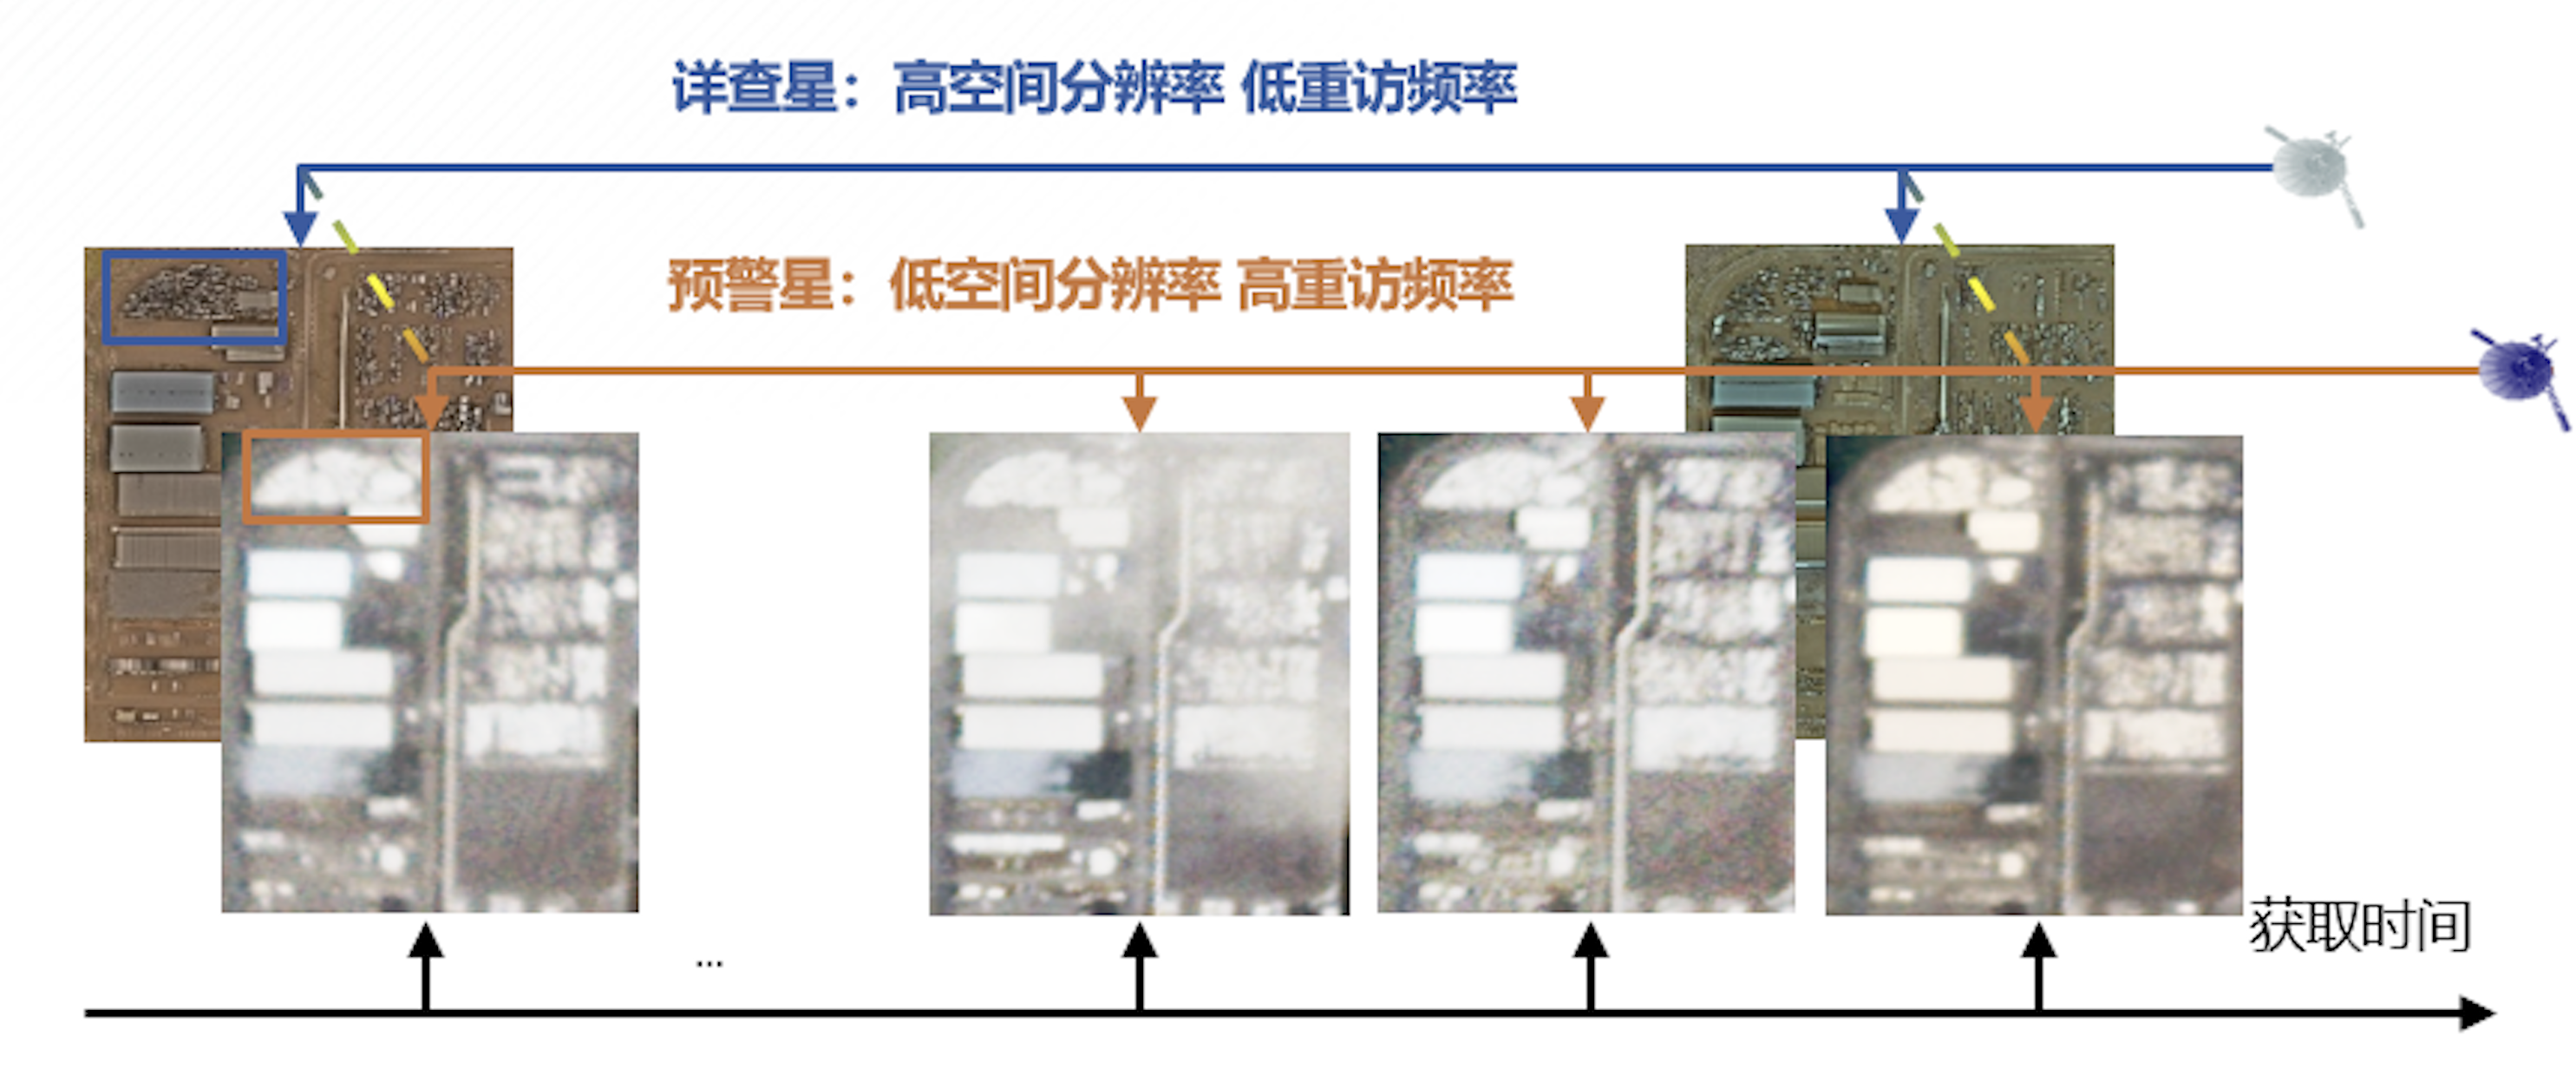
\includegraphics[width=\textwidth]{dataset.png}
    \caption{数据集概览}
    \label{fig:dataset}
\end{figure} 

其中LR 图像是www.planet.com 下载的,由 PlanetScope 卫星拍摄,地面分辨率为每像素 3m。为了起到监督作用,HR 图像是在根据相应 LR 图像的日期选择的,这些图像是从 WorldView 捕获的,地面分辨率为每像素 30 厘米。


\subsubsection{数据集分析}  
\begin{figure}[H]
    \centering
    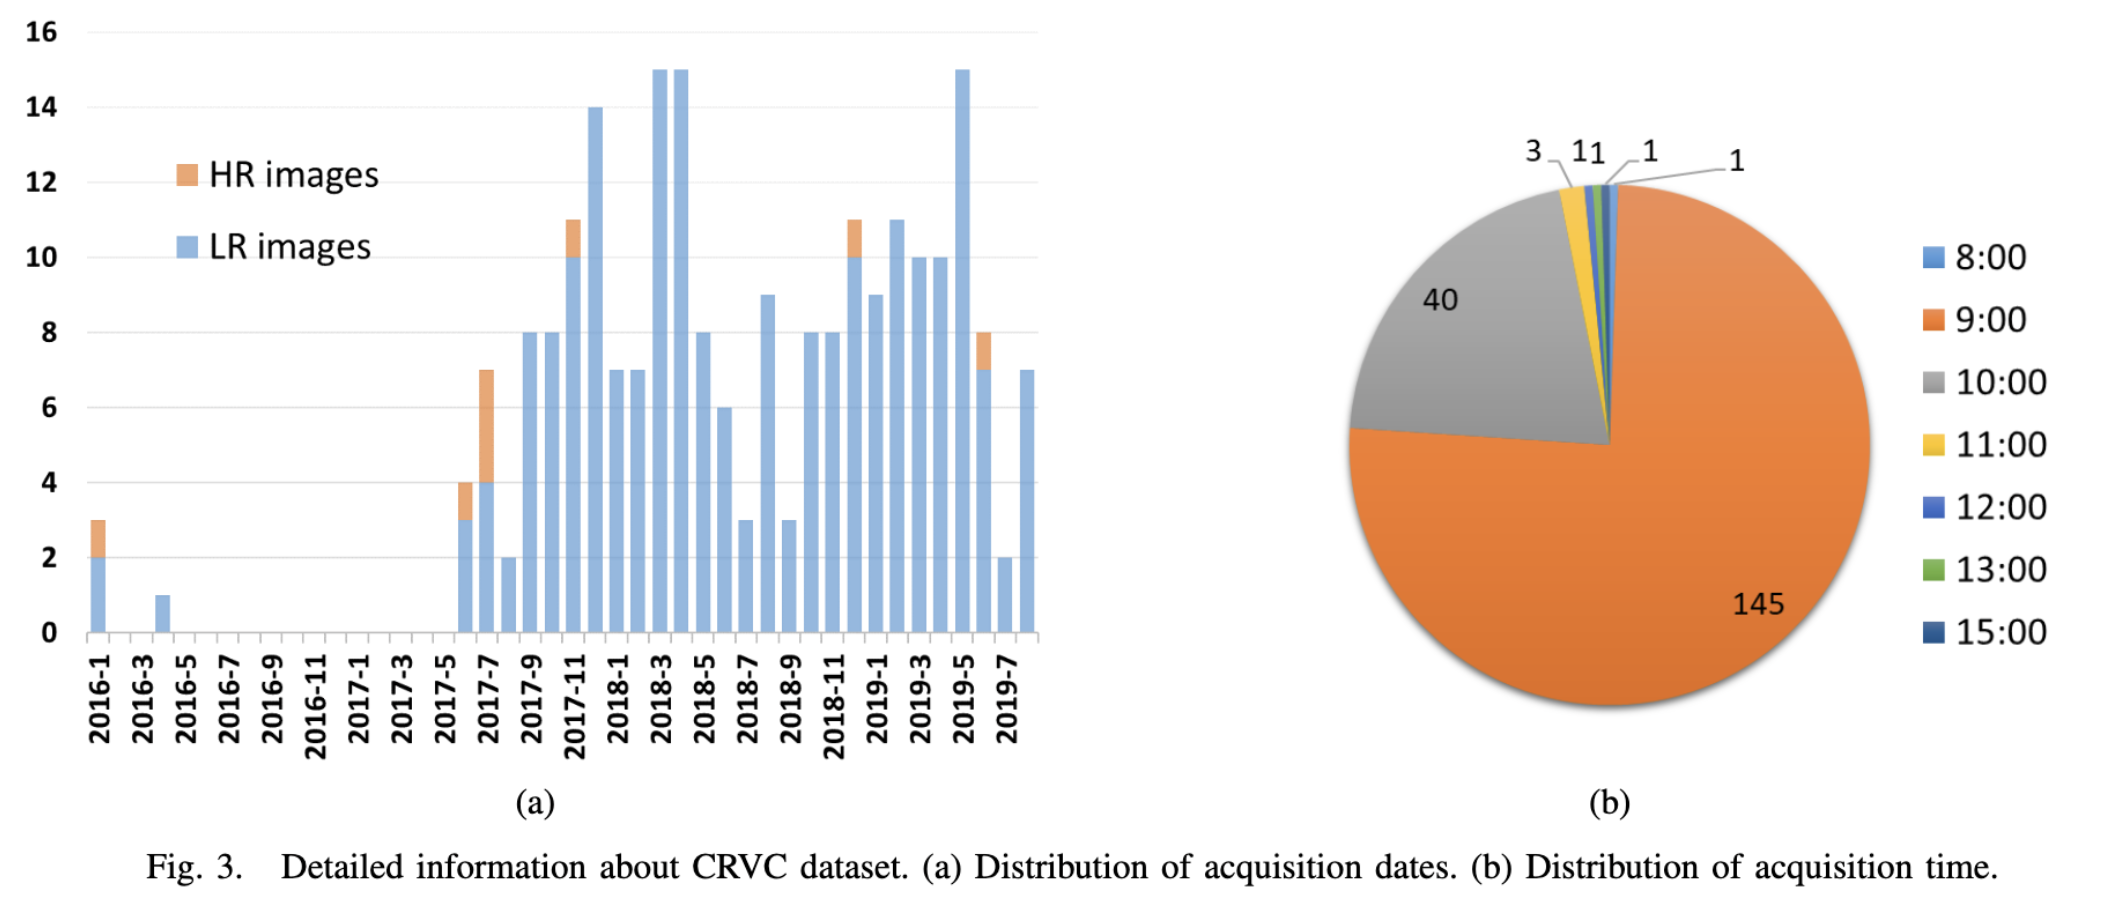
\includegraphics[width=\textwidth]{CRVCtime.png}
    \caption{数据的日期和时间分布}
    \label{fig:CRVCtime}
\end{figure}
图 ~\ref{fig:CRVCtime} 显示了数据集中LR和HR图像采集的日期和时间分布。可以观察到,数据的分布并不平均,主要集中在2017年5月至2019年7月之间。就8张高分辨率图像的日期而言,它们之间的时间间隔最小为 6 天,最大为 17 个月。 如表格~\ref{tab:date}中数据所示,HR 图像和相应 LR 图像之间的采集时间并不完全一致,平均采集时间差异为 39 分钟。在这种情况下,我们认为短时间内的HR和LR图像中的车辆数目一致。这一假设和实际情况相符并大大降低了建模难度。 
\begin{table}[h]
    \centering
    \caption{HR和LR图像的获取日期与时间}
    \label{tab:date}
    \begin{tabularx}{\textwidth}{CCCC}
      \toprule
      日期 & HR拍摄时间 & LR拍摄时间  \\
      \midrule
      4th January, 2016    & 10:56  &10:36\\
      26th June, 2017      &10:24   & 9:34\\
      2nd July, 2017       &10:20   & 9:36\\
      9rth July, 2017      &10:34   & 9:44\\
      15th July, 2017      &10:30   & 9:41\\
      9th November, 2017   &10:25   & 9:42\\
      19th December, 2018  &10:46   & 9:56\\
      6th June, 2019       &10:35   &10:29\\
      \bottomrule
    \end{tabularx}
\end{table}


\subsubsection{高分辨率图像处理}  
为了进行计数任务,该数据集在HR图像上标注了车辆的边界及类别。HR图像上标注框的数量作为对应日期的LR图像的真值。标注的边界则作为停车场位置的空间提示信息。该数据集中总共注释了 37852 个车辆实例,包含四类车辆,包括轿车、小型卡车、大型卡车和起重机(图~\ref{fig:vehicle})。不同类别的车辆在尺寸形状上有着很大的不同,分类计数有助于提升计数质量。  各类车辆数量极不平衡,分别为轿车35844辆、小型货车737辆、大型货车1211辆、起重机60辆。 
\begin{figure}[h]
    \centering
    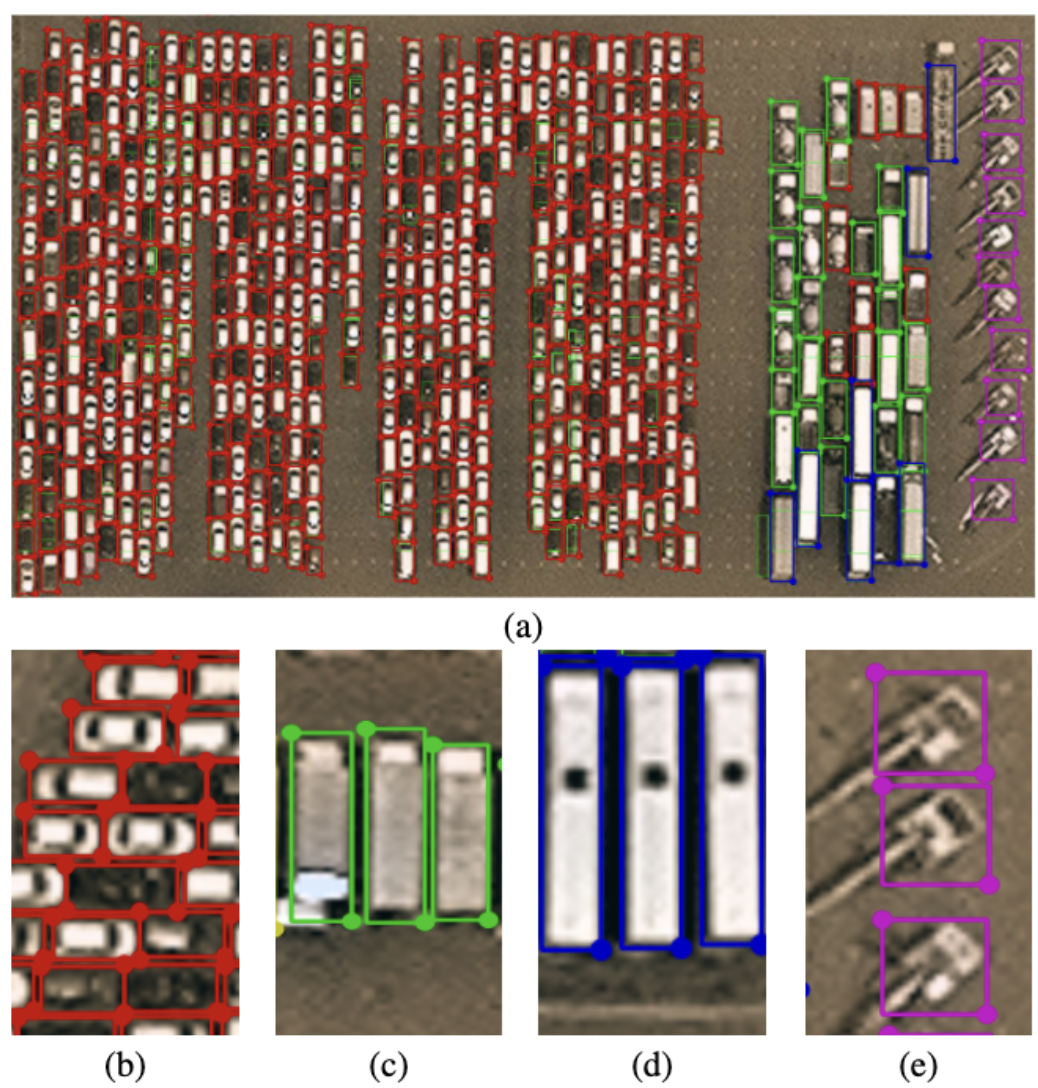
\includegraphics[width=0.5\textwidth]{vehicle.png}
    \caption{HR图像车辆标注及分类}
    \label{fig:vehicle}
\end{figure}

\subsubsection{低分辨率图像处理}  
数据集中共包含192张低分辨率图像。这些图像在2016至2019年之间被采集,主要分布在2017年6月至2019年8月之间,其中61.5\%的采集间隔在两天以内。如图~\ref{fig:CRVCtime}所示,低分辨率图像的采集时间均为日间,大部分图像拍摄于上午9点到10点。我们可以认为这些图像具有相似的拍摄条件。
不同于高分辨率图像,低分辨率图像的标注要困难的多。因为难以在低分辨率的条件下辨认清晰的车辆轮廓,所以标注车辆覆盖率是一个更可行的方法。由于低分辨率图像的视场较大,车辆区域只占图像中很小的一部分。因此先在HR图像中划出9个区域(图~\ref{fig:9parkHR}),在LR图像中对应位置进行覆盖率估计(图~\ref{fig:9parkpair})。
\begin{figure}[h]
    \centering
    \begin{subfigure}{0.45\textwidth}
        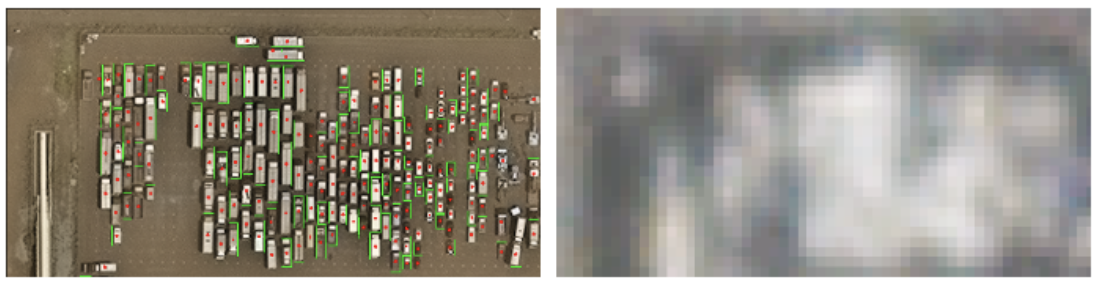
\includegraphics[width=\linewidth]{9parkpair.png}
        \caption{区域2对应的HR和LR图像}
        \label{fig:9parkpair}
    \end{subfigure}
    \begin{subfigure}{0.45\textwidth}
      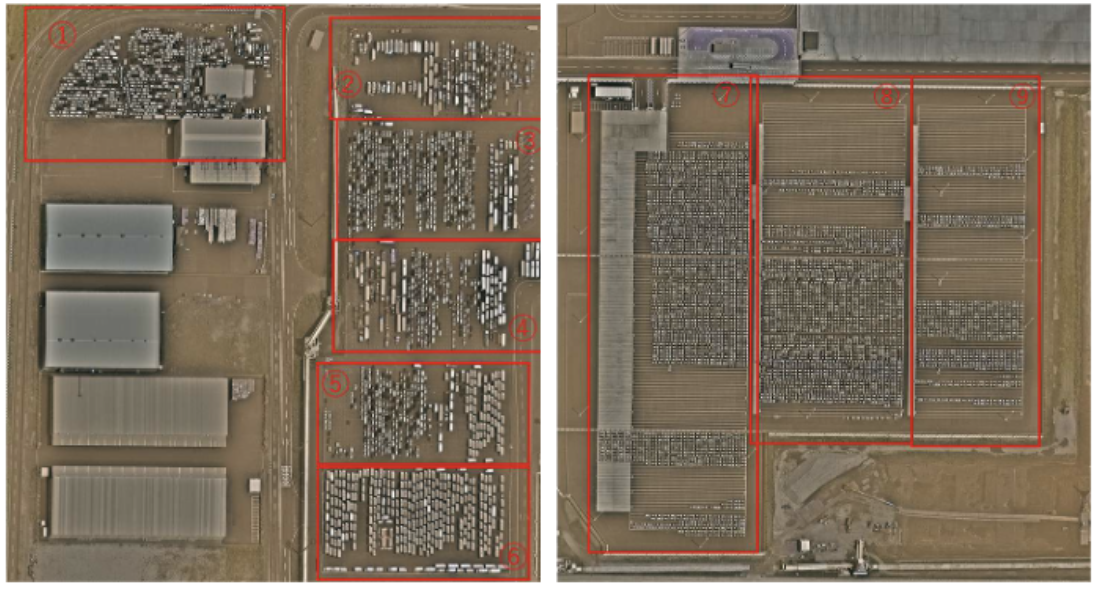
\includegraphics[width=\linewidth]{9parkHR.png}
      \caption{9个停车区域}
      \label{fig:9parkHR}
    \end{subfigure}\quad % 添加一些间隔
    
\end{figure}

% \begin{figure}[h]
%     \centering
%     \begin{subfigure}{\textwidth}
%         \centering
%         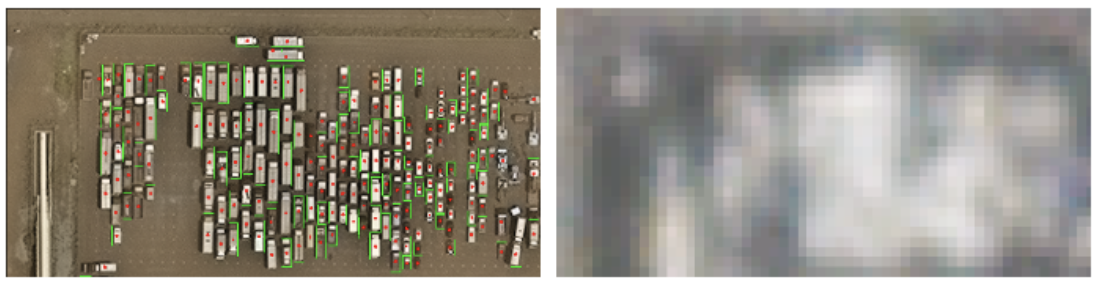
\includegraphics[width=0.6\linewidth]{9parkpair.png} % 调整宽度以适应你的需求
%         \caption{区域2对应的HR和LR图像}
%         \label{fig:9parkpair}
%     \end{subfigure}
    
%     \begin{subfigure}{\textwidth}
%       \centering
%       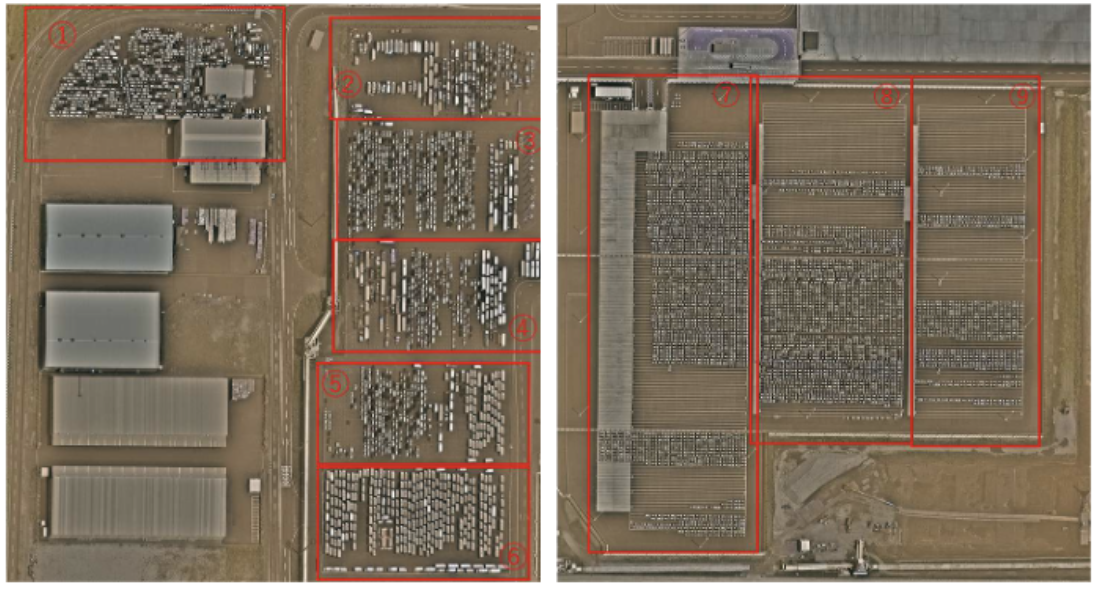
\includegraphics[width=0.6\linewidth]{9parkHR.png} % 调整宽度以适应你的需求
%       \caption{9个停车区域}
%       \label{fig:9parkHR}
%     \end{subfigure}
    
%     % \caption{这是两个子图的总标题。}
%     \label{fig:combinedfigure}
% \end{figure}



低分辨率图像可以分为两类,有对应高分辨率图像的和没有对应高分辨率图像的。对于前者而言,直接从对应高分辨率标注结果中计算覆盖率即可。那些没有HR图像对应的LR图像则由多名专家进行视觉标注并取平均值。


\subsubsection{数据集特性分析}  
通过上述对数据集的分析,我们可以看到高分辨率图像和与其对应的低分辨率图像之间间隔时间不大,同时对应的是同一位置。因此我们可以认为在它们上进行的目标计数结果应当也相同。两者所映射的空间信息应该具有一致性,这也给后续处理方法提供了思路。如何应用高分辨率图像信息指导改进低分辨率图像上估计的结果成为提高估计精度的关键节点之一。

同时单一的低分辨率图像很难得出合理的目标计数估计,然而由于低分辨率遥感图像的短重访周期,我们能得到一段连续的低分辨率图像。比较相邻图像间的变化或者从多个图像间进行学习,可以补充那些单张图像因低分辨率造成的信息缺失。图像间的时间连续性也是指导改进图像计数估计结果的关键因素。

\section{研究目标与内容}
\subsection{研究目标}
\begin{enumerate}    
    \item 跨分辨率车辆计数算法的开发:开发一种新的基于深度学习的车辆计数算法,该算法能够有效利用有限的高分辨率图像来指导低分辨率图像中的车辆计数。
    \item 探究高效利用数据集中空间一致性和时间连续性信息的方式:探究同一时刻高分辨率与低分辨率图像间的空间一致性和连续低分辨率图像间的时间连续性的高效利用方式。研究不同分辨率图像对算法效果的具体影响。
    \item 探究注意力机制在跨分辨率目标计数的应用:探索注意力机制在提高跨分辨率车辆计数准确性中的应用,尤其是如何通过注意力机制来增强模型综合多种特征表示的能力。
\end{enumerate}

\subsection{研究内容}
\begin{enumerate}
    \item 研究背景与意义分析:分析相关遥感技术的发展背景,高分辨率与低分辨率遥感图像的特点及其在车辆计数中的面临困难和挑战。梳理了当前目标检测、语义分割、基于回归和密度图的计数方法等方面的研究进展,特别关注跨分辨率图像处理及车辆计数领域的最新研究成果。
    \item 跨分辨率车辆计数数据集分析:对CRVC数据集进行分析调研,了解其数据组成分布以及数据中隐含的性质的分析及建模。
    \item 基于注意力机制的车辆计数模型设计:设计并实现一种新的基于注意力机制的深度学习模型,用于提高跨分辨率遥感图像车辆计数的准确性。
    \item 算法的性能评估及优化:在CRVC数据集上评估设计算法的性能,进行消融实验,并与现有的车辆计数方法进行比较。进一步优化算法,以达到更高的计数准确性和更好的泛化能力。
\end{enumerate}

\section{章节安排}
第一章为绪论,整体介绍研究背景及研究内容。第二章为目标计数方法计数框架,详细解释了目标计数领域的方法细节。第三章介绍了基于注意力机制的跨分辨率遥感影像计数方法,详细解释了基于注意力机制的深度学习网络设计细节。第四章设计了多组实验从分割精度、覆盖率估计和回归计数结果这三个方面测试了模型的性能。第五章对本设计做出总结和展望。

% Chapter 2

\chapter{目标计数基础理论和技术框架}
\section{深度学习基础理论}
目前主要的目标识别以及计数方法基于深度学习模型设计的,本小节介绍本文模型涉及到的深度学习相关理论。
\subsection{卷积层}
对于CRVC数据集中的图像数据,常使用卷积层\cite{minaee2021image,2012ImageNetClassificationDeepConvolutionalNeuralNetworks}来进行特征提取。卷积层具有的平移不变性和局部性非常适合处理图像数据,可以掌握图像的空间特征。下面给出卷积层的基本定义。
\begin{equation}
  \label{eq:eq_conv-layer}
  [\mathbf{H}]{i, j} = u + \sum_{a = -\Delta}^{\Delta} \sum_{b = -\Delta}^{\Delta} [\mathbf{V }]{a, b} [\mathbf{X}]_{i+a, j+b}
\end{equation}
通过使用系数$[\mathbf{V}]{a, b}$对位置$(i, j)$附近的像素$(i+a, j+b)$进行加权得到$[\mathbf{H}]{i, j}$。 其中$|a|> \Delta$或$|b| > \Delta$约束条件使得该式满足局部性,即只关注于在位置像素$(i+a, j+b)$的小领域范围内的参数,大大减少了参数量。$\mathbf{V}$被称为卷积核(convolution kernel)或者滤波器(filter),也是该卷积层的权重,通常该权重是可学习的参数。参数a,b也对应着卷积核的尺寸$k_h,k_w$。

上式\eqref{eq:eq_conv-layer}是单通道情况下卷积层的数学表示,当输入图像的通道数为$c_i$时,那么我们需要构造一个形状为$c_i\times k_h\times k_w$的卷积核。由于输入和卷积核都有$c_i$个通道,我们可以对每个通道输入的二维张量和卷积核的二维张量进行互相关运算,再对通道求和得到一个二维张量。这就是一个输出通道的结果。如果我们需要输出通道数为$c_o$时,只需创建一个卷积核的形状是$c_o\times c_i\times k_h\times k_w$。通道数量可以视作对于不同特征的描述,随着神经网络层数的加深,通常的做法是减少空间分辨率的同时增加通道数量。

\subsection{填充和步幅}
在应用多层卷积时,我们常常丢失边缘像素。填充(padding)可以解决这个问题。在输入图像的边界填充一定数量的元素(通常填充元素是$0$)。  
通常,如果我们添加$p_h$行填充(大约一半在顶部,一半在底部)和$p_w$列填充(左侧大约一半,右侧一半),则输出形状将为

\begin{equation}
  (n_h-k_h+p_h+1),(n_w-k_w+p_w+1)
\end{equation}
这意味着输出的高度和宽度将分别增加$p_h$和$p_w$。
在许多情况下,我们可以设置$p_h=k_h-1$和$p_w=k_w-1$,这样使得输入和输出具有相同的高度和宽度。假设$k_h$是奇数,我们将在高度的两侧填充$p_h/2$行。 如果$k_h$是偶数,通常会在输入顶部填充$\lceil p_h/2\rceil$行,在底部填充$\lfloor p_h/2\rfloor$行。同理,我们填充宽度的两侧。

感受野是指卷积网络中某一层输出特征图上的一个元素所对应的输入图像上的区域大小。它表征着特征图能“看到”的区域的大小。我们可以通过连续的卷积来增加感受野,但这会增加参数量。我们还可以通过调整步幅来增大感受野。
步幅是卷积操作中卷积核移动的步长。在对图像进行卷积时,卷积核从图像的一个角落开始,按照指定的步幅在图像上滑动,每次移动指定的像素数,直到覆盖整个图像。当步幅大于1时,卷积核每次移动多个像素,输出的特征图的尺寸也会随之减小。具体公式如下:

通常,当垂直步幅为$s_h$,水平步幅为$s_w$时,输出形状为
\begin{equation}
  \lfloor(n_h-k_h+p_h+s_h)/s_h\rfloor \times \lfloor(n_w-k_w+p_w+s_w)/s_w\rfloor
\end{equation}
如果我们设置了$p_h=k_h-1$和$p_w=k_w-1$,则输出形状将简化为$\lfloor(n_h+s_h-1)/s_h\rfloor \times \lfloor(n_w+s_w-1)/s_w\rfloor$。 更进一步,如果输入的高度和宽度可以被垂直和水平步幅整除,则输出形状将为$(n_h/s_h) \times (n_w/s_w)$。

\subsection{激活函数}
卷积神经网络中常用的激活函数包括ReLU(线性整流单元)\cite{2018DeepLearningusingRectifiedLinearUnitsReLU}、Sigmoid\cite{han1995influence}、Tanh(双曲正切)\cite{apicella2021survey}等。这些激活函数的目的是在网络中引入非线性特性,使得网络能够学习到更加复杂的数据表示。本文用到的是 线性整流函数ReLU (Rectified Linear Unit)函数和Sigmoid函数。
对于给定元素$x$,ReLU函数被定义为该元素与$0$的最大值。它是目前最常用的激活函数之一。因为它的导数在大于0时为1,小于0时为0,这使得它可以用来缓解梯度消失的问题。
\begin{equation}
  f(x) = \max(0, x)
\end{equation}

Sigmoid函数将输入值映射到(0, 1)区间,这常常用于分类预测或者给出概率预测。然而,由于其在输入值绝对值较大时梯度接近0,可能会导致梯度消失问题。
\begin{equation}
  f(x) = \frac{1}{1 + e^{-x}}
\end{equation}

\subsection{池化层}
池化(pooling)\cite{2022ComparisonPoolingMethodsConvolutionalNeuralNetworks}是卷积神经网络中常见的一种方法,主要用于减少特征图的维度,减少计算量的同时保留重要的一致性信息。与卷积层类似,池化运算也是通过一个固定形状的窗口滑动来实现的。与之不同的是,池化通过对邻近像素进行统计学操作(如取最大值或平均值)来实现,因此也不包含参数。主要有两种类型的池化:平均池化(Average Pooling)\cite{2022ComparisonPoolingMethodsConvolutionalNeuralNetworks}和最大池化(Max Pooling)\cite{2011Maxpoolingconvolutionalneuralnetworksvisionbasedhandgesturerecognition}
池化操作通常有两个参数:池化核的大小(\(K \times K\))和步幅(S)。池化核指定了池化操作的邻域范围,步幅定义了池化操作的移动间隔。对于输入大小为$W \times H$的特征图,池化操作后的输出大小$W' \times H'$可以通过以下公式计算:
\begin{equation}
  W' = \left\lfloor\frac{W - K}{S} + 1\right\rfloor
\end{equation}
\begin{equation}
  H' = \left\lfloor\frac{H - K}{S} + 1\right\rfloor
\end{equation}

在卷积网络的实践中,池化层通常有降低特征维度、引入不变性、增加鲁棒性和防止过拟合的作用。

\subsection{权重衰减}
在模型训练时,可能会遇到过拟合的问题,使得模型在已有数据上有着较好的性能,而在测试数据上表现不佳。我们可以使用多种正则化技术来缓解过拟合的问题。权重衰减(weight decay)\cite{2012L2RegularizationLearningKernels}是最广泛使用的正则化的技术之一, 它通常也被称为$L_2$正则化。
$L_2$ 正则化在损失函数中添加模型权重的平方之和作为惩罚项。同时通过一个非负的超参数$\lambda$来控制正则化的强度。$L_2$正则化正则化修正后的损失函数如下式:
\begin{equation}
  L(\mathbf{w}, b)=\frac{1}{n} \sum_{i=1}^{n} \frac{1}{2}\left(\mathbf{w}^{\top} \mathbf{x}^{(i)}+b-y^{(i)}\right)^{2}+\frac{\lambda}{2}\|\mathbf{w}\|^{2}
\end{equation}

L2正则化的目的是鼓励模型学习到更小更分散的权重值,从而提高模型的泛化能力。它对大的权重值施加较大的惩罚,从而防止模型依赖于少数几个可能具有高噪声的特征。

\subsection{暂退法}
Dropout(暂退法)\cite{wu2021r}在训练过程中以一定几率随机“丢弃”(即暂时移除)网络中的一部分神经元(包括其连接),这有助于模型学习到更加鲁棒的特征,减少神经元间复杂的共适应关系。需要注意的是,在测试时,我们通常不使用dropout。
\subsection{批量归一化}
批量归一化(Batch Normalization)\cite{bjorck2018understanding}是通过对每个小批量数据进行归一化处理,调整神经网络中间层的输出,使其均值接近0,标准差接近1。这可以通过减去它们的均值除以它们的标准差得到。这有助于稳定和加速深度网络的训练过程,同时也具有一定的正则化效果。
批量归一化(Batch Normalization,简称BN)是一种在深度神经网络中广泛使用的技术,用于加速训练过程并提高模型的稳定性。其基本思想是在网络的每层之后添加一个归一化步骤,这个步骤会对每个小批量数据(mini-batch)进行归一化处理,以确保网络中间层的激活分布保持稳定。批量归一化的公式如下:

\begin{equation}
  \hat{x}_i = \frac{x_i - \mu_B}{\sqrt{\sigma_B^2 + \epsilon}} 
\end{equation}
其中,$\epsilon$是一个很小的数,用来防止除以零。归一化后的\(\hat{x}_i\)具有零均值和单位方差。
\section{目标计数}
目前目标计数领域主要有三类方法。一类是检测方法\cite{girshick2014rich,girshick2015fast,ren2015faster,redmon2016you,redmon2017yolo9000,he2017mask},通过目标检测模型识别出具体的物体位置,之后根据结果来进一步计数。但这类方法对于输入图像的分辨率有着较高的要求,往往需要物体具有明确清晰的边缘特征。在低分辨率下往往表现效果较差。一种是基于回归的方法\cite{2009BayesianPoissonRegressionCrowdCounting,2013MultisourceMultiscaleCountingExtremelyDenseCrowdImages,2009CrowdCountingUsingMultipleLocalFeatures},直接拟合出图像特征和目标数目之间的回归模型得到图像中对应物体的数目。但这种方法未能完整利用图像中的空间位置信息和时间序列信息。当输入图像的大小和分布有变化的情况下,往往不具有很强的泛化能力。另一类方法是基于密度图的目标计数方法\cite{li2018csrnet,2016SingleImageCrowdCountingMultiColumnConvolutionalNeuralNetwork,2018CrowdCountingusingDeepRecurrentSpatialAwareNetwork,2018VehicleDetectionCountingHighResolutionAerialImagesUsingConvolutionalRegressionNeuralNetwork}。此类方法通常先得出一个目标物体在区域内的一个分布,之后就可以通过密度分布来估计总体的数量。该方法在稠密计数的场景下往往具有较好的效果。在本文使用的跨分辨率车辆计数数据集上,可以把车辆计数视为一个稠密计数场景。使用基于密度图的计数方法相较其余两类方法有着更好的表现。受上述方法启发,本文将跨分辨率车辆计数问题转换为两个子问题,即综合跨分辨率图像信息的图像分割网络和映射分割结果和最终计数目标的回归模型。

\section{U-Net网络}
U-Net
\cite{cheng2021transfer}是一个广泛被应用的语义分割模型,最初被应用于医学图像的分割问题上。U-Net是一个具有对称结构的网络,通过使用跳跃连接(Skip Connection)来结合低层次的位置信息和高层次的语义信息,从而在细节上进行更准确的预测。
\begin{figure}[h]
  \centering
  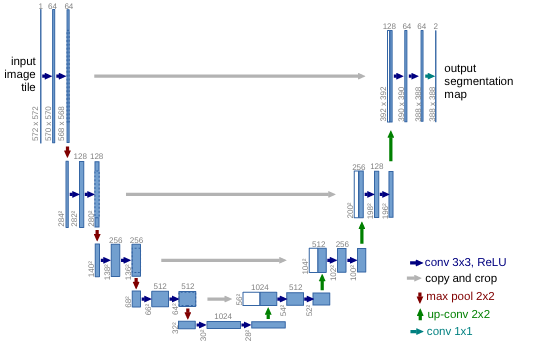
\includegraphics[width=\textwidth]{Unet.png}
  \caption{U-Net网络结构}
  \label{fig:UNet}
\end{figure}
\subsection{模型结构}
U-Net网络由一个收缩路径(contracting path)和一个扩展路径(expansive path)组成.网络的输入是一张$572\times 572$的的图片(input image tile)。网络最终的输出为同样尺寸的分割图预测。图像经过收缩路径提取综合特征,并保留中间特征信息。在扩展路径中,综合上采样后前一层特征结果与对应尺度的编码特征 ,得到最终的结果。因为整个网络结构形似字母‘U’,因此称为U-Net。
\subsection{收缩路径}
收缩路径是由多个卷积层、线性整流函数单元(ReLU)和最大汇聚层(Max Pooling)构成的一系列降采样操作。论文中将这一部分叫做压缩路径(contracting path)。压缩路径由4个块组成,每个块使用了3个有效卷积和1个Max Pooling进行下采样。每个块处理之后特征图的通道数扩大为2倍,特征图的长和宽也有相应缩小。这样的处理使得不同的特征被逐步提取到不同的通道中。最终得到了尺寸为$32\times 32$的特征图。
\subsection{扩展路径}
扩展路径是相同数量的相似模块组成。不同的是扩展路径中使用了反向卷积和上采样。同时扩展路径通过跳跃连接从收缩路径对应的层中获取特征图,并与当前层的特征图进行融合。这种结构有助于恢复图像的精细信息,使得在深度网络中消失的某些信息不至被遗忘。
在深度学习和计算机视觉中,上采样(Upsampling)和反向卷积(也称为转置卷积,Transposed Convolution)是两种常用的技术,用于增加图像或特征图的分辨率。这两种技术常见于像U-Net这样的网络结构中,用于从深层特征映射中恢复图像的细节信息,尤其在图像分割和生成模型中十分重要。

\subsection{双线性插值}
上采样是一种用于增加图像或特征图的尺寸的方法。它通过已有数据的插值来增加分辨率,主要有最近邻插值、双线性插值和双三次插值等方法。下面主要介绍双线性插值\cite{2022Upsamplingcomparativestudynewideas}。
在双线性插值中,输出像素的值是输入像素值的加权平均,权重基于像素之间的距离。假如我们想得到未知函数 f 在点 $P=\left( x, y\right)$ 的值,假设我们已知函数 f 在 $Q_{11} = \left( x_1, y_1 \right) $, $Q_{12} = \left( x_1, y_2 \right) $, $Q_{21} = \left( x_2, y_1 \right) $, 及 $Q_{22} = \left( x_2, y_2 \right) $ 四个点的值。 

首先在 x 方向进行线性插值,得到:
\begin{align}
f(x, y_1) &\approx \frac{x_2-x}{x_2-x_1} f(Q_{11}) + \frac{x-x_1}{x_2-x_1} f(Q_{21}), \\
f(x, y_2) &\approx \frac{x_2-x}{x_2-x_1} f(Q_{12}) + \frac{x-x_1}{x_2-x_1} f(Q_{22}).
\end{align}

然后在 y 方向进行线性插值,得到 
\begin{equation}
  \begin{aligned}
    f(x,y) &\approx \frac{y_2-y}{y_2-y_1} f(x, y_1) + \frac{y-y_1}{y_2-y_1} f(x, y_2) \\
&= \frac{y_2-y}{y_2-y_1} \left ( \frac{x_2-x}{x_2-x_1} f(Q_{11}) + \frac{x-x_1}{x_2-x_1} f(Q_{21}) \right ) \\
&+ \frac{y-y_1}{y_2-y_1} \left ( \frac{x_2-x}{x_2-x_1} f(Q_{12}) + \frac{x-x_1}{x_2-x_1} f(Q_{22}) \right ) \\
&= \frac{1}{(x_2-x_1)(y_2-y_1)} \big( f(Q_{11})(x_2-x)(y_2-y)+ f(Q_{21})(x-x_1)(y_2-y)\\
&+  f(Q_{12})(x_2-x)(y-y_1) + f(Q_{22})(x-x_1)(y-y_1) \big)\\
&=\frac{1}{(x_2-x_1)(y_2-y_1)}  \begin{bmatrix} x_2-x & x-x_1 \end{bmatrix} \begin{bmatrix} f(Q_{11}) & f(Q_{12}) \\ f(Q_{21})& f(Q_{22}) \end{bmatrix} \begin{bmatrix}
y_2-y \\ y-y_1 \end{bmatrix}.
  \end{aligned}
\end{equation}

如果先在 y 方向插值、再在 x 方向插值,其结果与按照上述顺序双线性插值的结果是一样的。由上式我们不难看出,双线性插值由两个线性函数的积构成,因此为网络带来了非线性。

\subsection{转置卷积}

转置卷积\cite{2018guideconvolutionarithmeticdeeplearning}是一种更复杂的上采样技术,它通过神经网络来试图学习一种更有效的插值方式。它不仅增加了特征图的尺寸,还可以学习在上采样过程中引入新的信息。它通过反转卷积操作的流程实现,因此被称为转置卷积。
标准卷积操作是将卷积核应用于多个输入上,得到一个输出,实际上就是建立了一个多对一的关系。对于转置卷积而言,我们实际上是想建立一个逆向操作,也就是建立一个一对多的关系。对于标准卷积,我们有:
\begin{equation}
𝑌=𝐶𝑋
\end{equation}

转置卷积其实就是要对其进行逆操作,求出X
\begin{equation}
  X=C^T Y
\end{equation}
假设输入特征图大小为\(W \times H\),卷积核大小为\(K \times K\),步长为\(S\),填充为\(P\),输出特征图大小可以通过以下公式计算:

\[ W' = S(W-1) + K - 2P \]
\[ H' = S(H-1) + K - 2P \]

这里\(W'\)和\(H'\)分别是输出特征图的宽度和高度。

\section{注意力机制}
注意力机制(Attention Mechanism)\cite{vaswani2017attention}是一种模仿认知注意力的机制。在认知科学中,由于信息处理的瓶颈,人类会选择性地关注信息中的某一一部分,同时忽略其他可见的信息。上述机制通常被称为注意力机制。随着该机制在Transformer\cite{vaswani2017attention}、BERT\cite{2018BERTPretrainingDeepBidirectionalTransformersLanguageUnderstanding}、GPT\cite{2023GenerativePretrainedTransformerComprehensiveReviewEnablingTechnologiesPotentialApplicationsEmergingChallengesFutureDirections}等NLP领域的成功,该机制及应用又成为了研究的热点话题。目前在计算机视觉领域,ViT\cite{2020ImageWorth16x16WordsTransformersImageRecognitionScale}、Flow1D\cite{2022ComparisonPoolingMethodsConvolutionalNeuralNetworks}等网络也都基于注意力机制进行设计。
从注意力的形式来分类的话,可以分为软注意力(soft attention)和硬注意力(hard attention)。其中软注意力机制是可微可导的,本文中主要探讨的也是软注意力机制。

\subsection{注意力机制基本原理}

\begin{figure}[h]
  \centering
  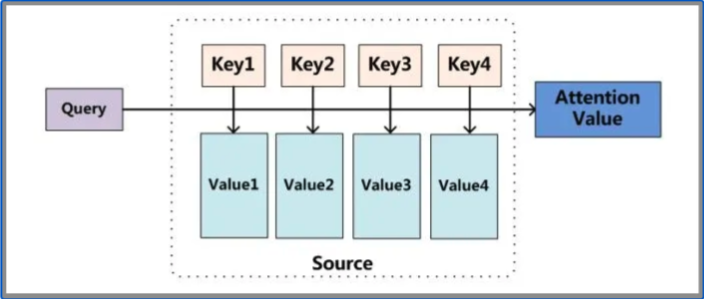
\includegraphics[width=\textwidth]{attention.png}
  \caption{注意力机制}
  \label{fig:attention}
\end{figure}

如图~\ref{fig:attention}所示,注意力机制主要涉及到3类数据,分别是键(key)、值(value)和查询(query)。当一个查询值到来时,计算查询和键的相似度,得到权重,并进行归一化处理。再将得到的权重和值加权求和得到我们最终的注意力结果。
首先计算查询与每个键之间的相似度。这一步通常使用点积(dot product)或者缩放点积(scaled dot product)来实现。具体来说,对于每个查询,通过计算它与所有键的点积,得到一个相似度分数:
\begin{equation}
  \text{score}(Q, K) = QK^T 
\end{equation}

接下来使用Softmax函数对上一步得到的相似度分数进行归一化,以确保所有的权重加起来等于1。:
\begin{equation}
   \text{Attention Weight} = \text{Softmax}(\text{score}(Q, K))
\end{equation}

用归一化后的权重对值进行加权求和,得到最终的注意力输出:
\begin{equation}
  \text{Output} = \text{Attention Weight} \cdot V 
\end{equation}

将上述步骤合并,注意力机制的输出可以通过以下公式计算:
\begin{equation}
\text{Attention}(Q, K, V) = \text{Softmax}\left(\frac{QK^T}{\sqrt{d_k}}\right)V 
\end{equation}

其中,\(d_k\)是键的维度,这个因子用于缩放点积,避免在维度很高时计算结果过大,导致Softmax函数处于饱和区,从而缓解梯度消失的问题\cite{vaswani2017attention}。
\subsection{注意力机制在图像领域的应用}
在图像处理领域中,使用注意力机制可以显著提升模型的性能,尤其是在图像分类、目标检测和图像分割等任务中。根据任务需要不同,常用的注意力机制有以下几种:
\begin{enumerate}    
  \item 空间注意力(Spatial Attention):关注图像的特定区域,通常用于增强模型对图像中重要部分的感知能力。可以用来替代传统的卷积网络,找到目标区域。
  \item 通道注意力(Channel Attention):关注不同通道的相关性,可以帮助模型识别哪些特征是更加重要的。
  \item 自注意力(Self-Attention):通过计算图像内所有位置之间的关系,可以捕捉更广泛的上下文信息。在时间序列模型中,自注意力机制可以保证长序列中的所有位置的信息有参与后续计算的可能。在图像领域中,对图像数据自身使用自注意力机制使得输出中每一位置均含有输入图像中所有位置的加权信息。
\end{enumerate}

在图像领域实践中,同时还使用以下几种训练策略:
\begin{enumerate}    
  \item 多尺度注意力:使用多尺度注意力可以帮助模型同时关注图像的粗略和详细特征,这在处理具有不同尺寸和形状的对象时特别有效。
  \item 融合不同的注意力机制:同时使用空间和通道注意力,或者将传统的注意力机制与自注意力结合起来,可以提取更丰富的特征并提高模型的性能。
  \item 注意力正则化:添加注意力正则化可以防止模型对某些特征过度依赖,从而提高模型的泛化能力。使用如残差连接等设计可以训练更深层的网络,防止训练过程中的信息丢失。
\end{enumerate}

\subsection{注意力机制处理序列图像}
在处理序列图像,如视频帧、时间序列的医学图像或连续的监控遥感数据时,我们不仅要考虑图像中的空间信息,也需要考虑图像间的序列信息。对于注意力机制的设计使用有着更高的要求。自注意力机制和多图像帧的相互注意力机制常常用来捕获时间和空间上的复杂关系。以下是这些注意力机制在序列图像处理中的一些常见应用方式:

自注意力机制可以用于分析序列图像中的时间依赖性,这对于识别视频中的动态事件或时间序列图像中的变化特别有效。
\begin{enumerate}    
  \item 时间自注意力:在处理视频或其他序列图像时,可以在时间维度上应用自注意力,以识别不同时间点图像帧之间的关键依赖关系。在视频帧序列中,模型可以学习到哪些帧之间具有高度相关性,这对于动作识别、事件检测等任务非常有用。
  \item 空间自注意力:在单个图像帧内部,可以应用空间自注意力来分析图像中不同区域之间的相互作用,对于解决目标检测和图像分割等任务有很大的帮助。
  \item 时空自注意力:结合时间和空间自注意力,可以同时考虑空间位置和时间演变的关系。这种方法可以用于复杂场景的动态解析,如多物体交互的场景。
\end{enumerate}

这些方法在处理动态场景解析和增强特征表示上有着不错的表现。在动态变化的场景中,模型可以使用多目标间的相互注意力来预测未来的状态。而通过计算不同目标之间的相互关系,可以获得更丰富的场景表示,这对于场景分类、事件检测等任务非常有帮助。


\section{Attention U-Net网络}
Attention U-Net\cite{oktay2018attention}是一种结合了注意力机制的UNet网络,最初被应用于医学图像的分割问题上。它在U-Net的架构上增加了Attention Gate注意力门使得模型能更好的聚焦在目标区域。
\begin{figure}[h]
  \centering
  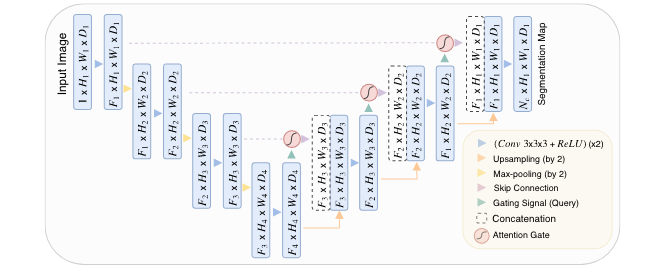
\includegraphics[width=\textwidth]{attention Unet.png}
  \caption{Attention U-Net}
  \label{fig:attentionunet}
\end{figure}

如图~\ref{fig:attentionunet}所示,Attention U-Net沿用了U-Net的基本架构,包括编码器(逐步下采样)和解码器(逐步上采样)两部分,以及跳跃连接(skip connections)来保留多尺度的特征。值得注意的是在每个跳跃连接处,新引入了注意力门控模块。这些模块对来自编码器的特征图进和解码器的相应特征图进行注意力计算。这使得网络能够聚焦于那些对最终分割任务更为重要的区域。

该方法将来自解码器的特征图作为查询,将来自编码器的特征图作为值和键作为注意力门的输入。注意力系数是通过一个小型的卷积网络学习到的,该网络计算当前解码器特征和对应编码器特征之间的相关性。
\begin{figure}[h]
  \centering
  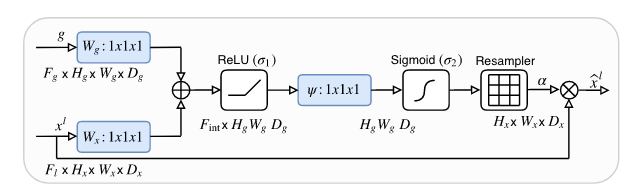
\includegraphics[width=\textwidth]{attention gate.png}
  \caption{Attention gate}
  \label{fig:attentiongate}
\end{figure}


在图~\ref{fig:attentiongate}中展示的是一个注意力门结构。注意力门接收两组输入,一组是来自上一下采样层的特征图(\(g\)),作为查询。另一组是来自跳跃连接的特征图(\(x^l\))键和值。
两组特征图首先通过一个\(1 \times 1 \times 1\)的卷积层(表示为\(W_g\)和\(W_x\)),这一步用于减少通道的数量,以降低后续计算复杂度。
接着,两组卷积后的特征图相加,并通过ReLU激活函数,得到\( \sigma_1\)。经过ReLU激活的特征图再次经过一个\(1 \times 1 \times 1\)卷积层,通常标识为\(\psi\),然后通过Sigmoid激活函数得到\( \sigma_2\),此时每个特征的激活值位于[0, 1]区间,代表了特征的重要性权重。将Sigmoid输出的权重与跳跃连接的特征图(\(x^l\))相乘。在这个过程中,三个\(1 \times 1 \times 1\)卷积层包含了我们需要学习的参数,也赋予了该模块掌握关键权重的能力。通过注意力门,我们得到了在解码器特征图做查询的情况下的加权编码器特征图。利用我们新得到的特征图来进行下一步解码,比原本单纯接受编码器输入获得了更丰富的信息。

\section{Flow1D网络}
Flow1D\cite{2022ComparisonPoolingMethodsConvolutionalNeuralNetworks}网络是一个基于注意力机制的光流估计网络。光流估计是计算机视觉中的一个基本问题,它旨在估计一幅图像上的每个像素点在时间序列中的运动,这在视频处理、运动分析、超分辨率、3D重建和自动驾驶等众多领域中都有广泛应用。光流估计是计算机视觉领域中的一个核心问题,光流是图像中像素点在时间维度上的瞬时运动速度和方向的场。光流是从连续的视频帧中估计出来的,这些连续的图像不仅具有时间上的连续性,光流也是从这些图像的空间关系中估计出来的。本文探讨的跨分辨率车辆计数问题,需要从同一时间的高分辨率低分辨率图像中找到空间一致性的关联,同时在连续的低分辨率图像中也要找到时间上的连续性关系。这和光流估计对于连续图像数据的利用有着不少相同之处。

\begin{figure}[h]
  \centering
  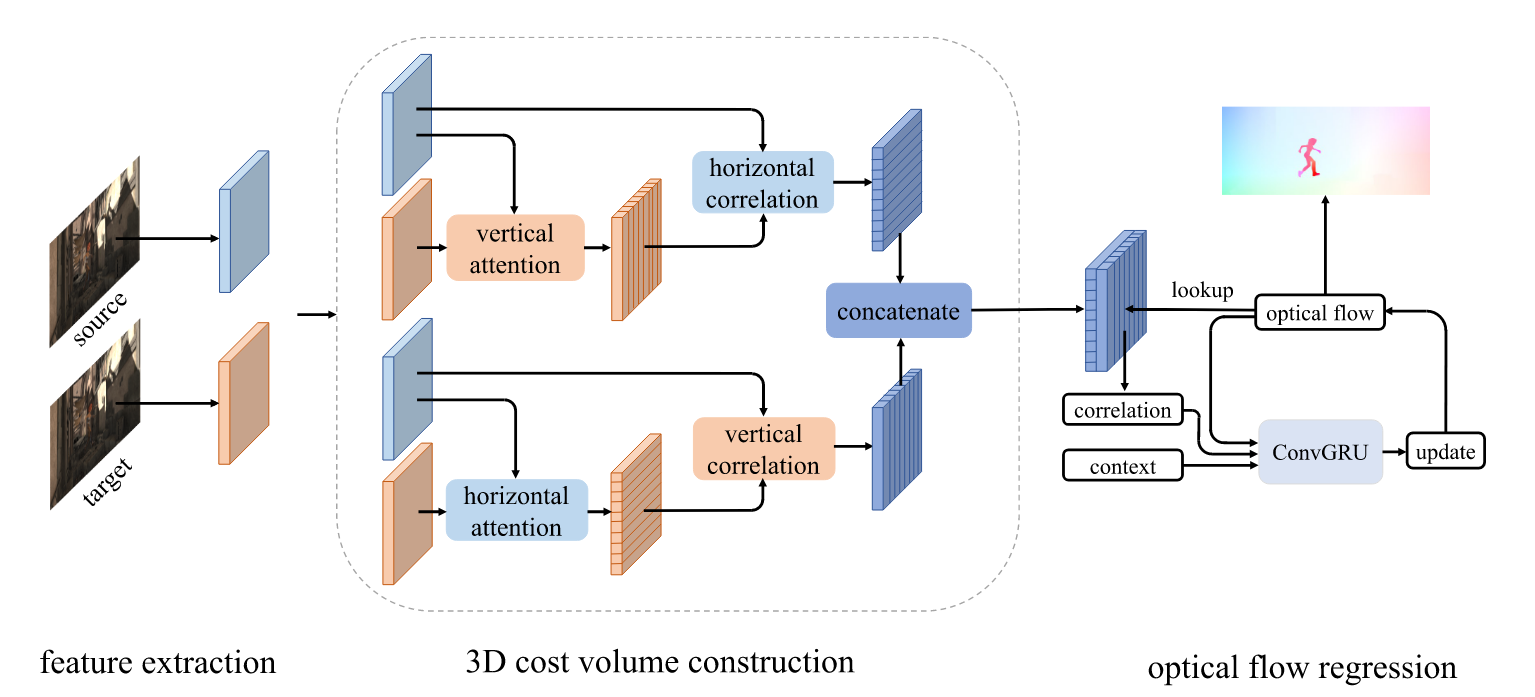
\includegraphics[width=\textwidth]{flow1d.png}
  \caption{Flow1D网络}
  \label{fig:Flow1D}
\end{figure}

图~\ref{fig:Flow1D}展示了模型的基本框架。对于源和目标两个图像,先分别进行特征提取,然后利用注意力机制计算3D cost volume。最后通过门控循环单元,通过相关性特征和初始提取出的特征,进行隐状态的计算。反复迭代计算出光流。
其中3D cost volume的设计充分利用了注意力机制的全局观察能力,通过两个一维的注意力操作,表征三维的光流状态。在水平竖直方向分别进行自注意力计算和相互之间的注意力计算。

\begin{figure}[H]
  \centering
  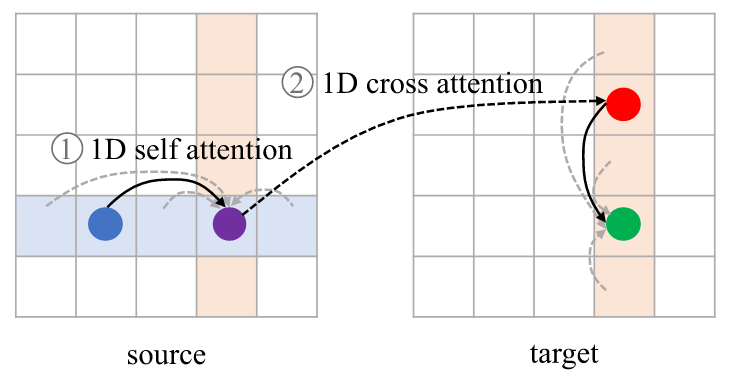
\includegraphics[width=\textwidth]{selfcross.png}
  \caption{self attention和cross attention}
  \label{fig:selfcross}
\end{figure}
图~\ref{fig:selfcross}是对注意力机制的一个很直观的展示。如果要计算源和目标的相关度,直接进行cross attention是不能得到红点与蓝点之间的相关关系的。因此需要再源上先进行self attention,使得每一个列向量包含着原先该列的一种加权分布。然后再进行cross attention操作,综合不同图像不同位置的信息。这是一种非常有效的策略。


\section{CRVC网络}
CRVC网络是针对CRVC数据集设计的深度学习模型。它以U-Net模型为骨架,针对跨分辨率空间CRVC数据集中的数据特性设计了两个分支来提取跨分辨率空间信息和时序信息。通过上述网络估计出密度分布后,使用线性回归模型得出最终目标计数结果。
\subsection{网络设计}

图~\ref{fig:CRVCnet}展示了模型的基本框架。模型接受4个输入,分别是高分辨率图像输入$I^{HR}$,对应低分辨率图像输入$I^{LR}$,与LR图像时间间隔较近的$I^{LR}_{near}$和与LR图像时间间隔较远的$I^{LR}_{far}$。模型包含两个独立学习的编码器HR encoder和LR encoder,前者用来提取高分辨率图像的特征,后者用来提取3个低分辨率图像的特征。提取出的低分辨率特征和高分辨率特征作差来综合更高精度的信息。之后通过带有跳跃连接的decoder完成分割图的生成。
\begin{figure}[h]
  \centering
  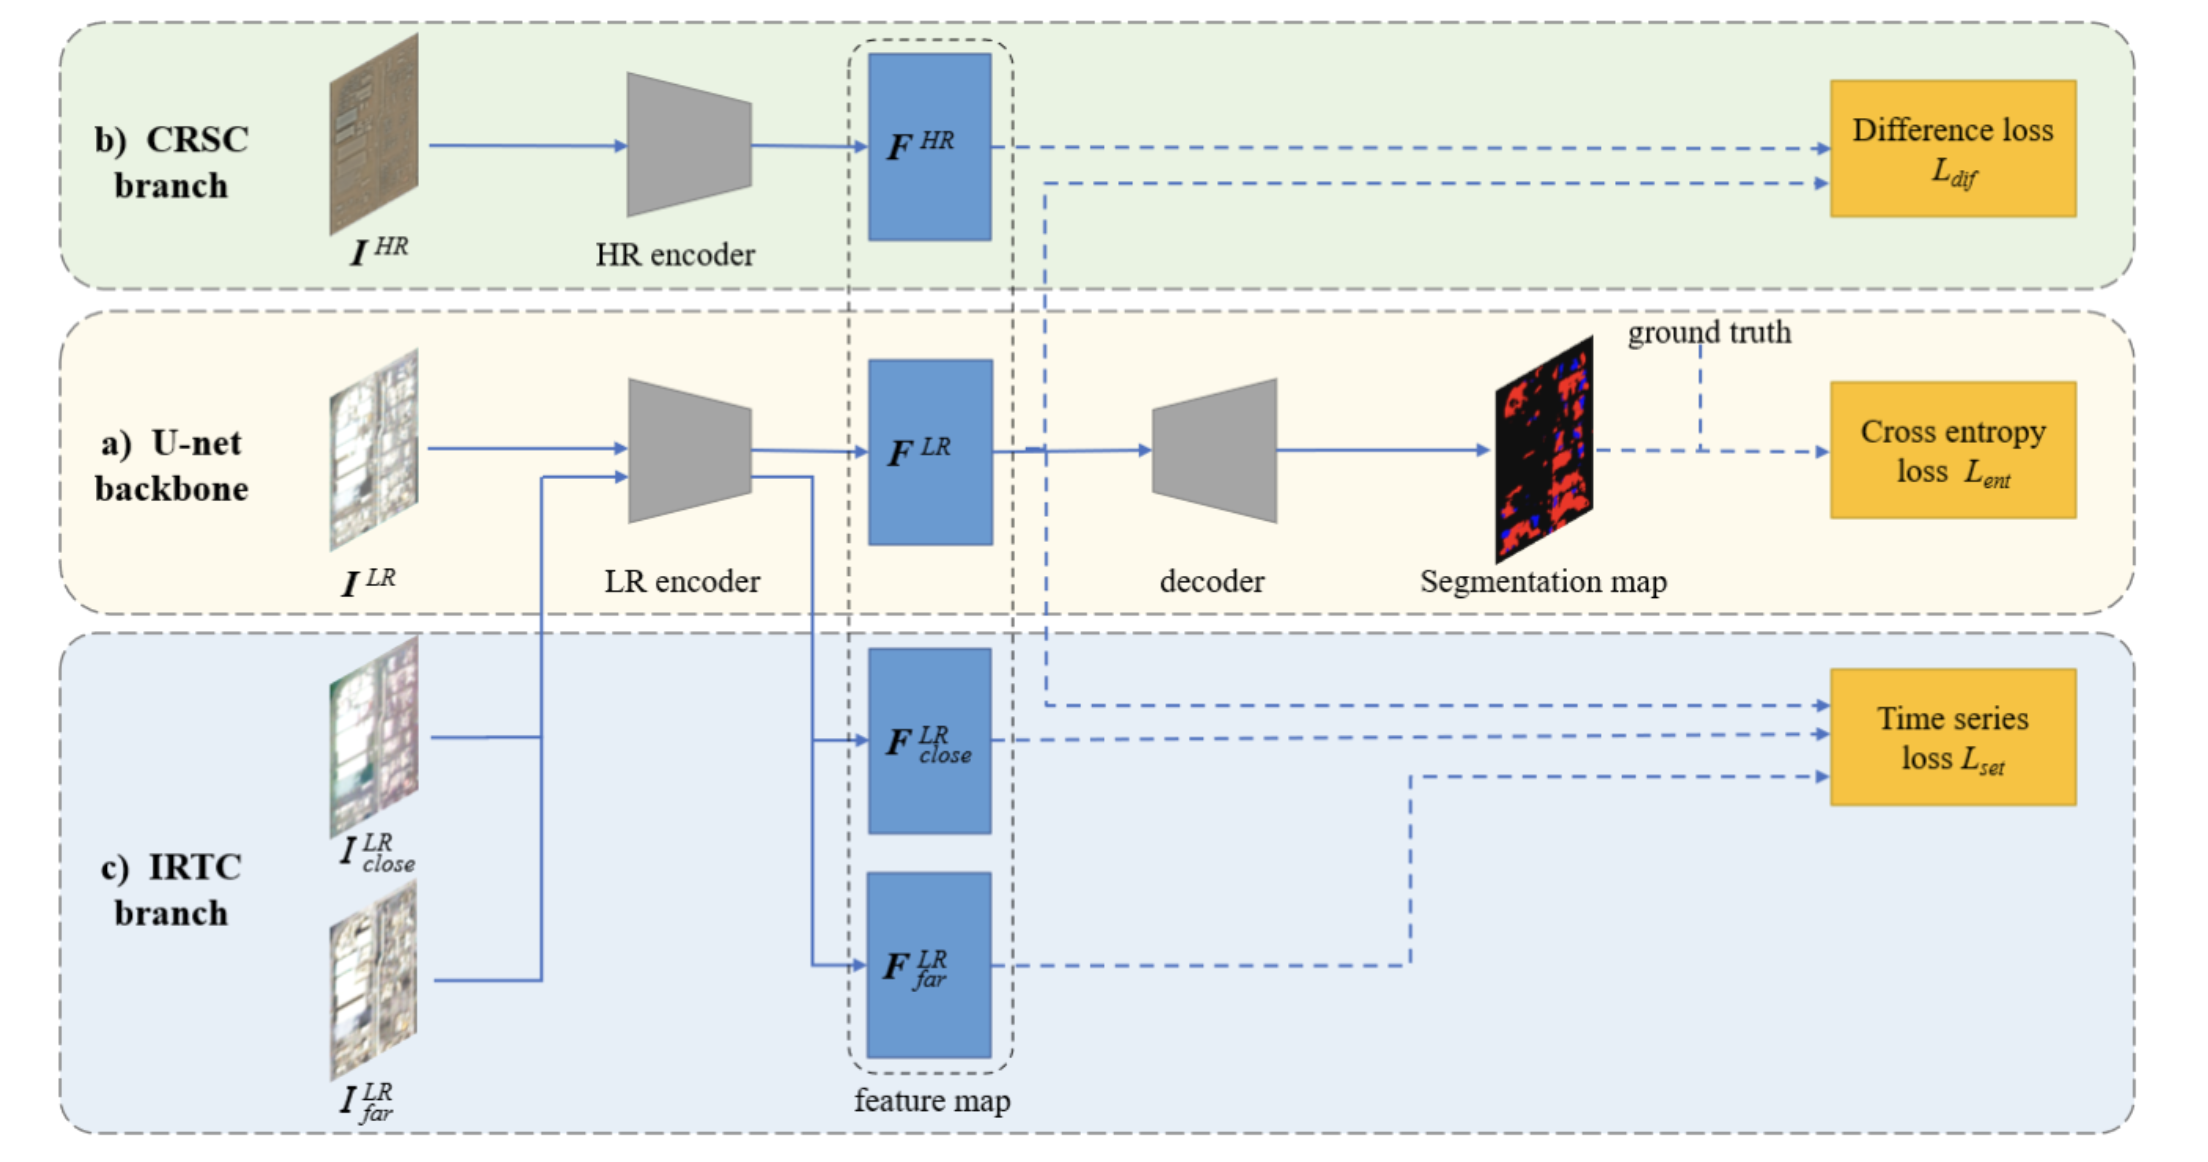
\includegraphics[width=\textwidth]{CRVCnet.png}
  \caption{CRVC网络架构}
  \label{fig:CRVCnet}
\end{figure}


\subsection{回归模型}

在CRVC数据集中,车辆在目标区域是密集停放的,而且不存在重叠。因此从分割图上估计出的覆盖率和最终的车辆数目具有线性关系。通过CRVC网络得到的覆盖率分割图,根据低分辨率图像的缩放比例,可以估计出实际面积。通过线性回归,找出参数k来拟合
\begin{equation}
    Number_i=k_i\dots Area_i+b_i
\end{equation}
其中i表示第i类车辆。这些参数通过高分辨率图像的真值计算得到。

\subsection{模型局限}
CRVC网络针对CRVC数据集的特点进行了设计,在各项评价指标上均优于传统目标计数方法。然而模型对于样本数量较少的类别的计数效果不是很理想。CRVC网络通过引入两个额外分支来分别提取高分辨率的空间信息和低分辨率的时序信息,然而,对于数据集中的时间连续性和空间一致性信息的挖掘,网络的表现仍有进一步优化的空间。本文针对上述问题进行了针对性设计。


% Chapter 3

\chapter{跨分辨率车辆计数数据集}

\section{数据集简介}
跨分辨率车辆计数数据集\cite{2022VehicleCountingVeryLowResolutionAerialImagesCrossResolutionSpatialConsistencyIntraresolutionTimeContinuity} 收集了日本常陆那珂港的 192 张极低分辨率图像和 8 张高分辨率图像,日期范围为 2016 年至 2019 年。\begin{figure}[h]
    \centering
    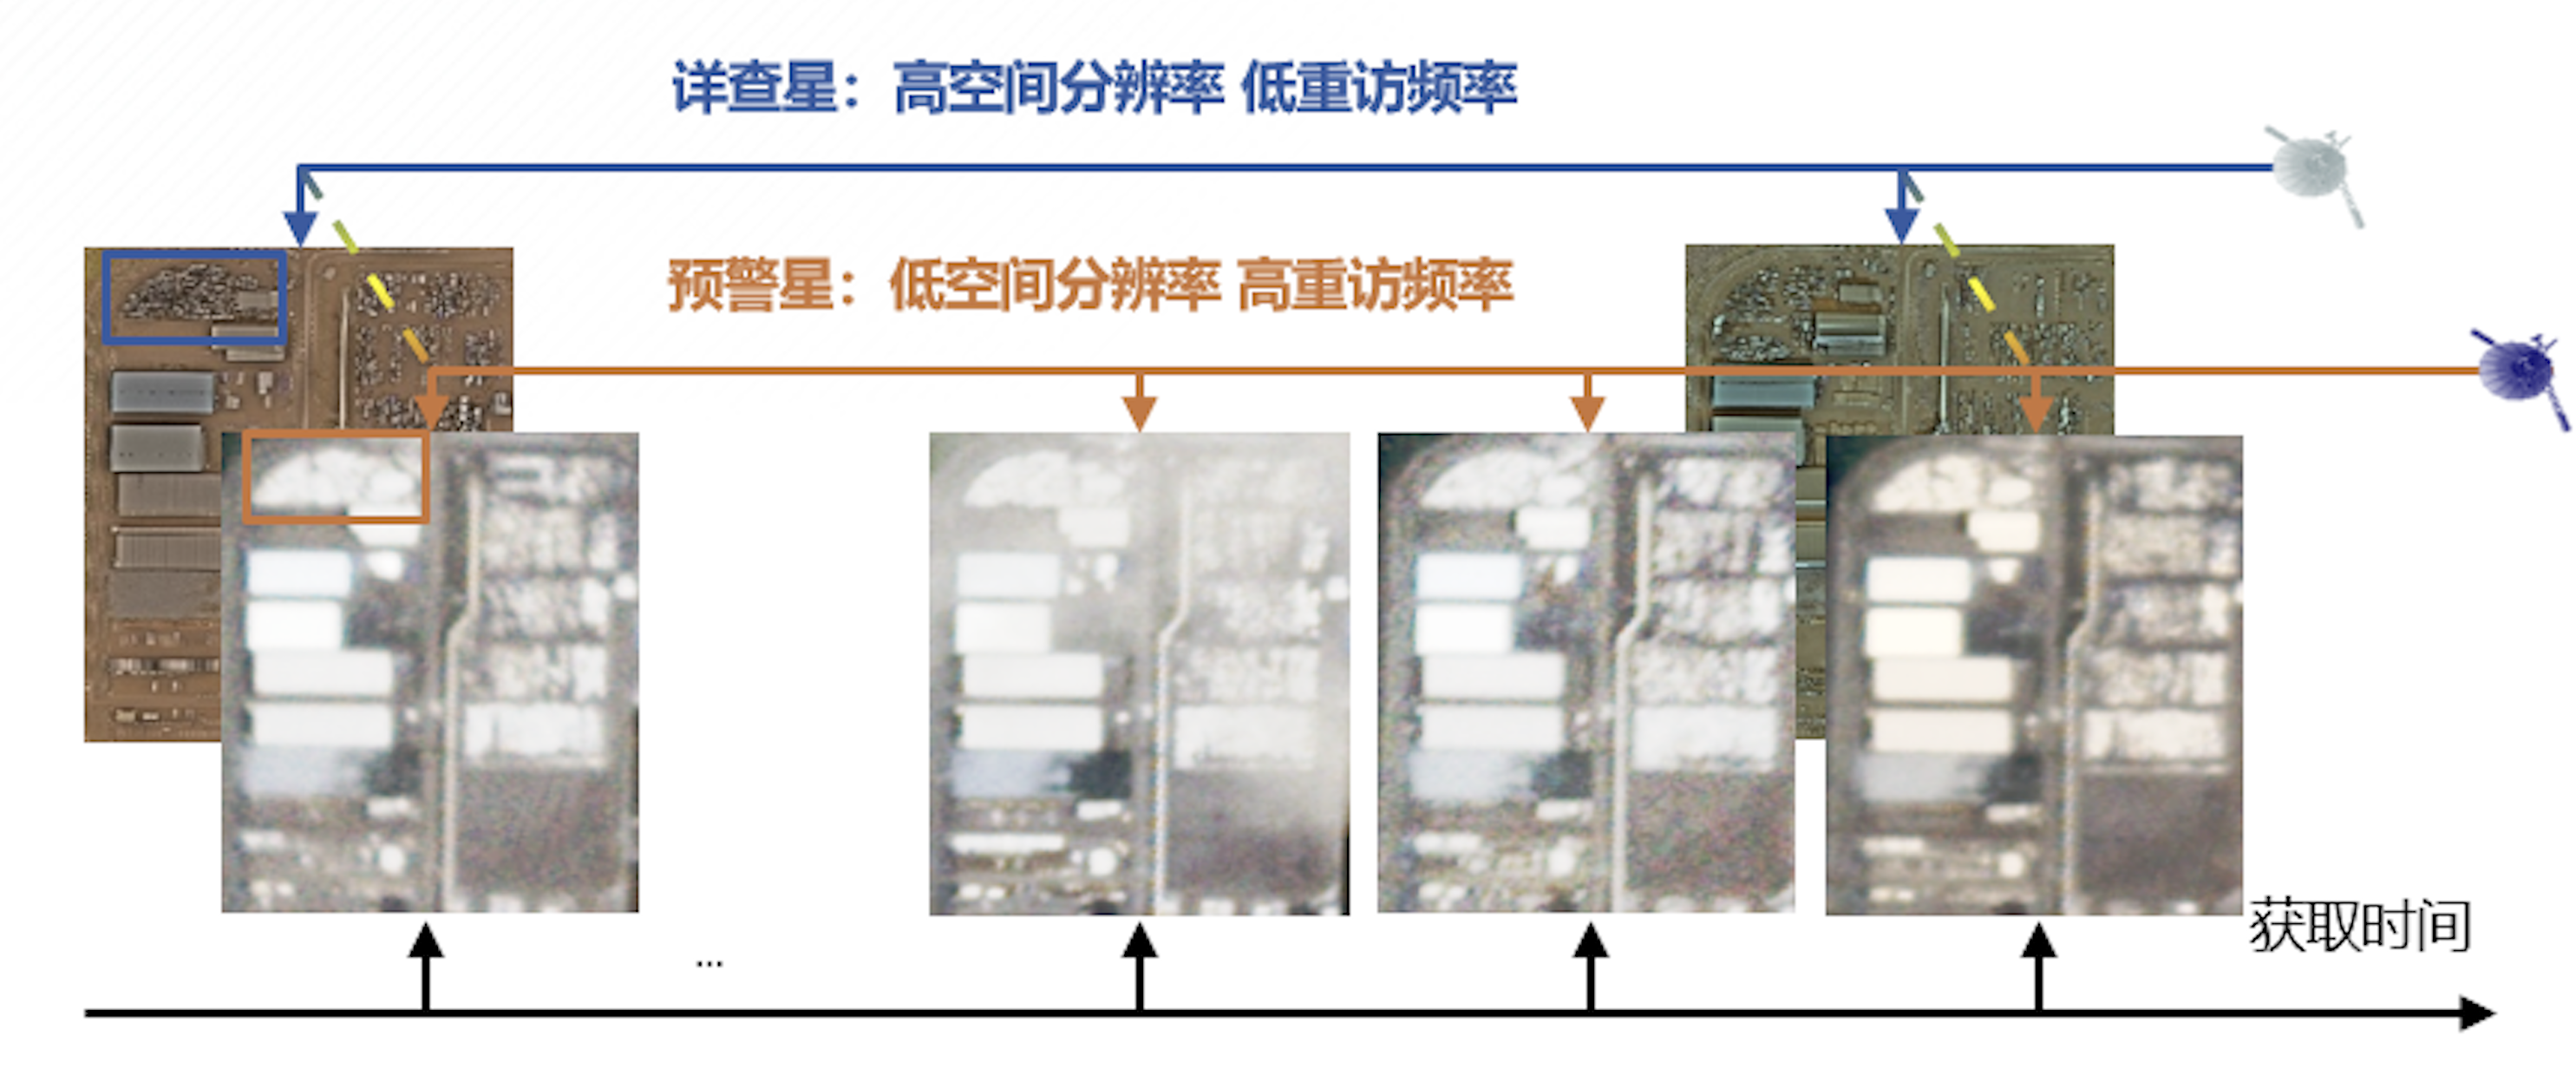
\includegraphics[width=\textwidth]{dataset.png}
    \caption{数据集概览}
    \label{fig:dataset}
\end{figure} 

其中LR 图像是www.planet.com 下载的,由 PlanetScope 卫星拍摄,地面分辨率为每像素 3m。为了起到监督作用,HR 图像是在根据相应 LR 图像的日期选择的,这些图像是从 WorldView 捕获的,地面分辨率为每像素 30 厘米。

\begin{figure}[h]
    \centering
    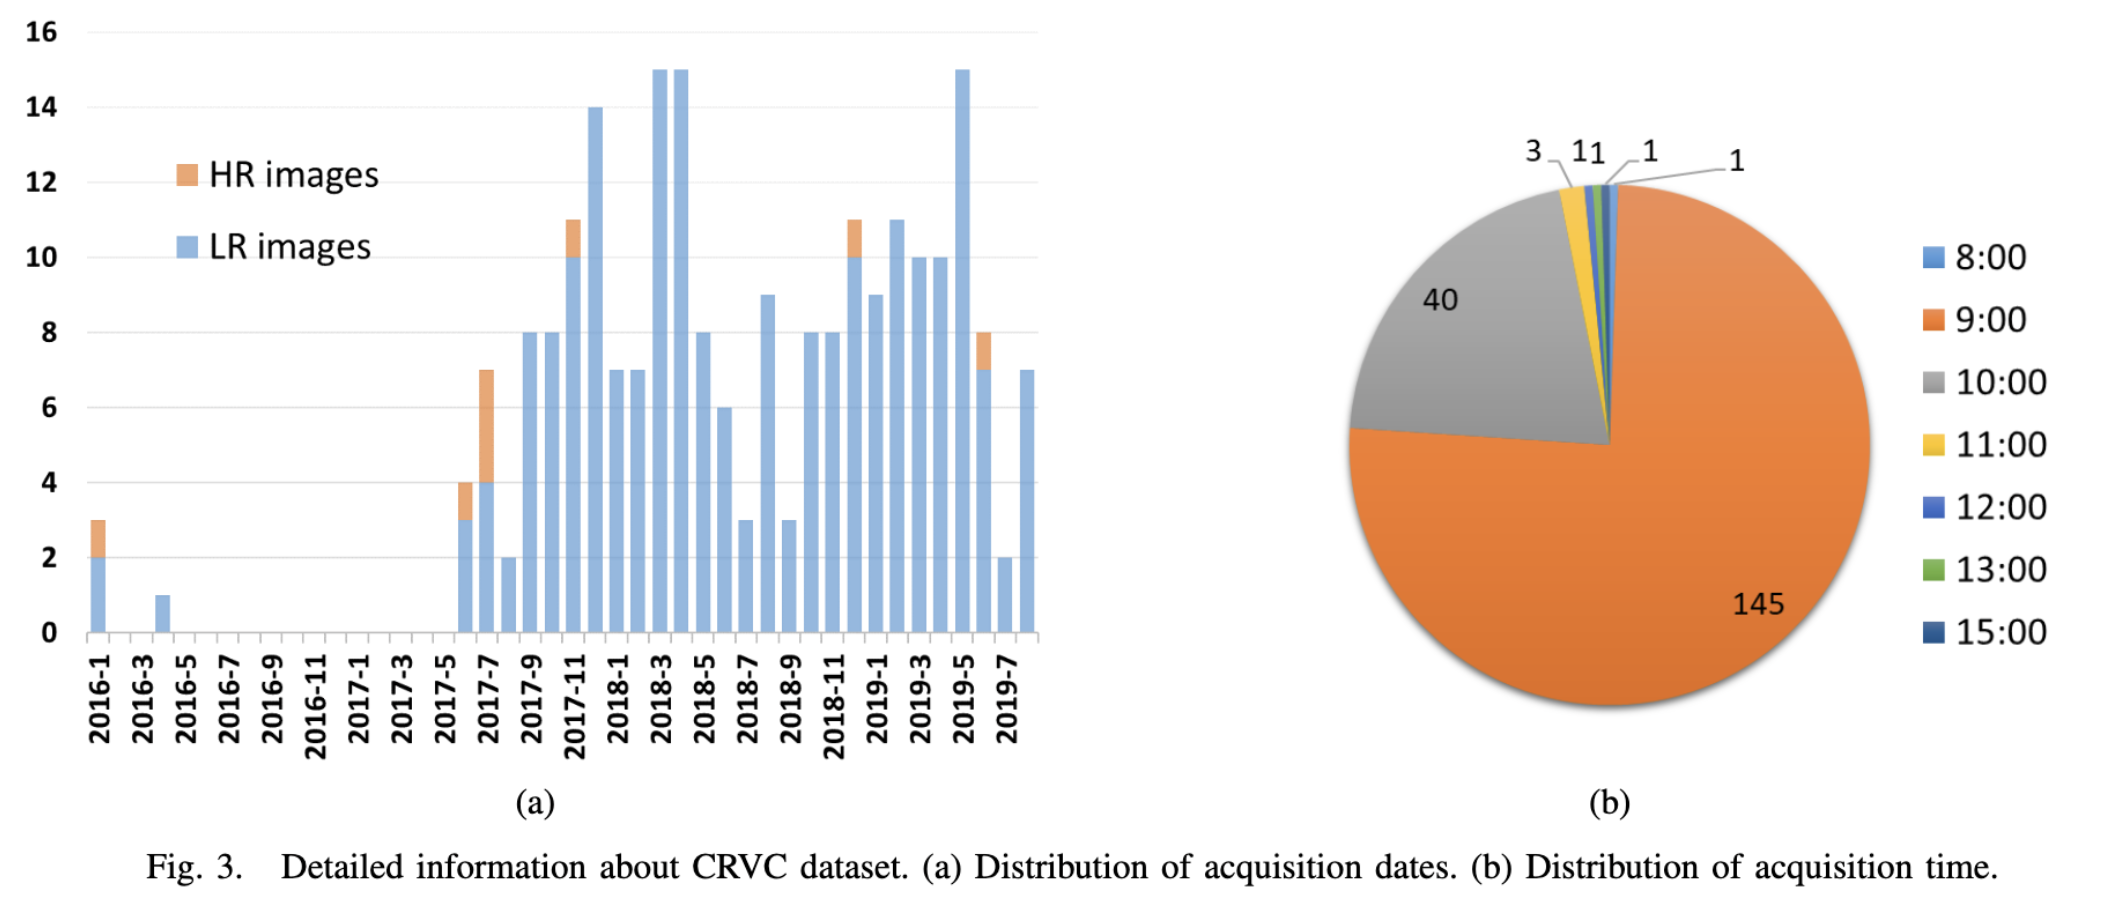
\includegraphics[width=\textwidth]{CRVCtime.png}
    \caption{数据的日期和时间分布}
    \label{fig:CRVCtime}
\end{figure}
\subsection{数据集分析}  
图 ~\ref{fig:CRVCtime} 显示了数据集中LR和HR图像采集的日期和时间分布。可以观察到,数据的分布并不平均,主要集中在2017年5月至2019年7月之间。就8张高分辨率图像的日期而言,它们之间的时间间隔最小为 6 天,最大为 17 个月。 如表格~\ref{tab:date}中数据所示,HR 图像和相应 LR 图像之间的采集时间并不完全一致,平均采集时间差异为 39 分钟。在这种情况下,我们认为短时间内的HR和LR图像中的车辆数目一致。这一假设和实际情况相符并大大降低了建模难度。 
\begin{table}[h]
    \centering
    \caption{HR和LR图像的获取日期与时间}
    \label{tab:date}
    \begin{tabularx}{\textwidth}{CCCC}
      \toprule
      日期 & HR拍摄时间 & LR拍摄时间  \\
      \midrule
      4th January, 2016    & 10:56  &10:36\\
      26th June, 2017      &10:24   & 9:34\\
      2nd July, 2017       &10:20   & 9:36\\
      9rth July, 2017      &10:34   & 9:44\\
      15th July, 2017      &10:30   & 9:41\\
      9th November, 2017   &10:25   & 9:42\\
      19th December, 2018  &10:46   & 9:56\\
      6th June, 2019       &10:35   &10:29\\
      \bottomrule
    \end{tabularx}
\end{table}


\subsection{高分辨率图像处理}  
为了进行计数任务,该数据集在HR图像上标注了车辆的边界及类别。HR图像上标注框的数量作为对应日期的LR图像的真值。标注的边界则作为停车场位置的空间提示信息。该数据集中总共注释了 37852 个车辆实例,包含四类车辆,包括轿车、小型卡车、大型卡车和起重机(图~\ref{fig:vehicle})。不同类别的车辆在尺寸形状上有着很大的不同,分类计数有助于提升计数质量。  各类车辆数量极不平衡,分别为轿车35844辆、小型货车737辆、大型货车1211辆、起重机60辆。 
\begin{figure}[h]
    \centering
    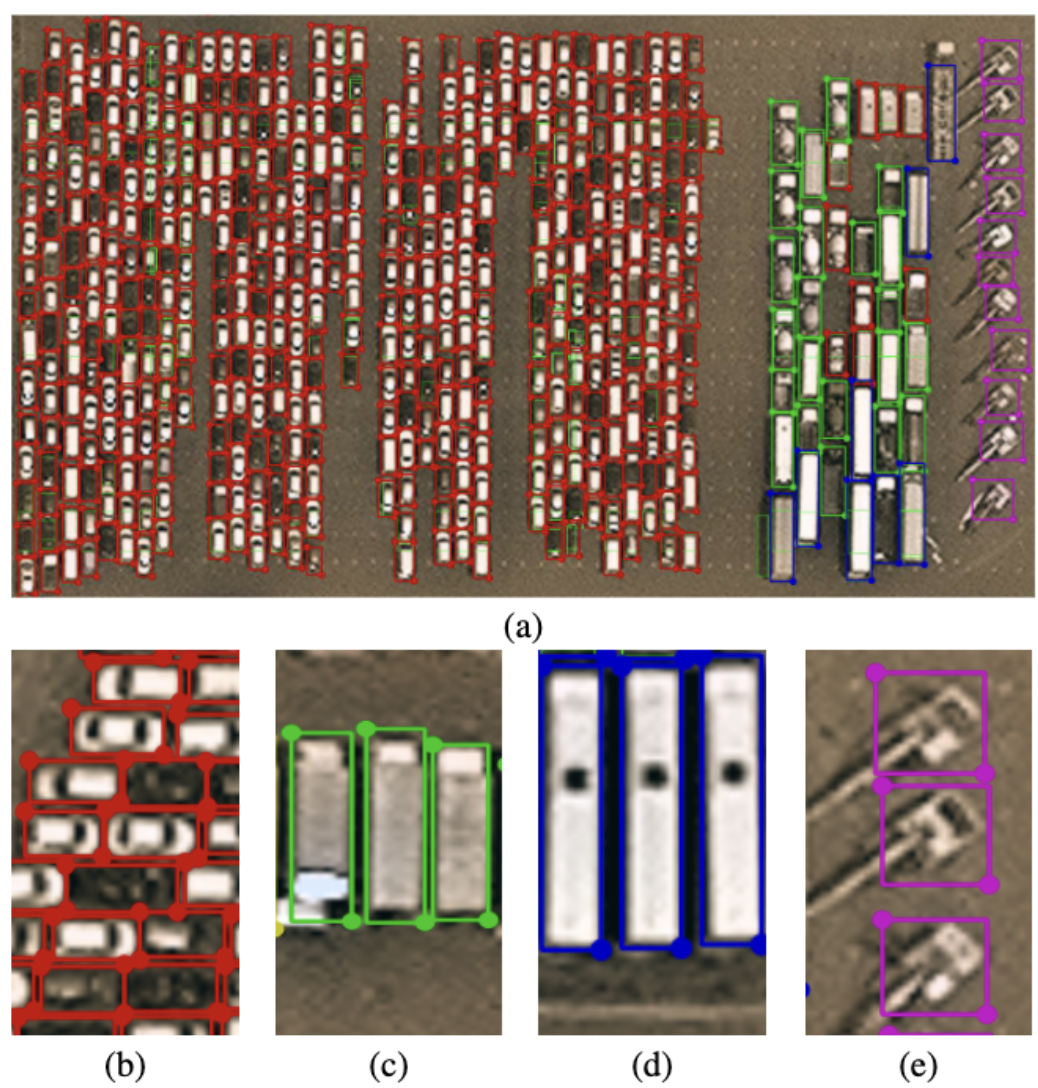
\includegraphics[width=0.5\textwidth]{vehicle.png}
    \caption{HR图像车辆标注及分类}
    \label{fig:vehicle}
\end{figure}

\subsection{低分辨率图像处理}  
数据集中共包含192张低分辨率图像。这些图像在2016至2019年之间被采集,主要分布在2017年6月至2019年8月之间,其中61.5\%的采集间隔在两天以内。如图~\ref{fig:CRVCtime}所示,低分辨率图像的采集时间均为日间,大部分图像拍摄于上午9点到10点。我们可以认为这些图像具有相似的拍摄条件。
不同于高分辨率图像,低分辨率图像的标注要困难的多。因为难以在低分辨率的条件下辨认清晰的车辆轮廓,所以标注车辆覆盖率是一个更可行的方法。由于低分辨率图像的视场较大,车辆区域只占图像中很小的一部分。因此先在HR图像中划出9个区域,在LR图像中的对应位置进行估计(图~\ref{fig:park})。
\begin{figure}[ht]
    \centering
    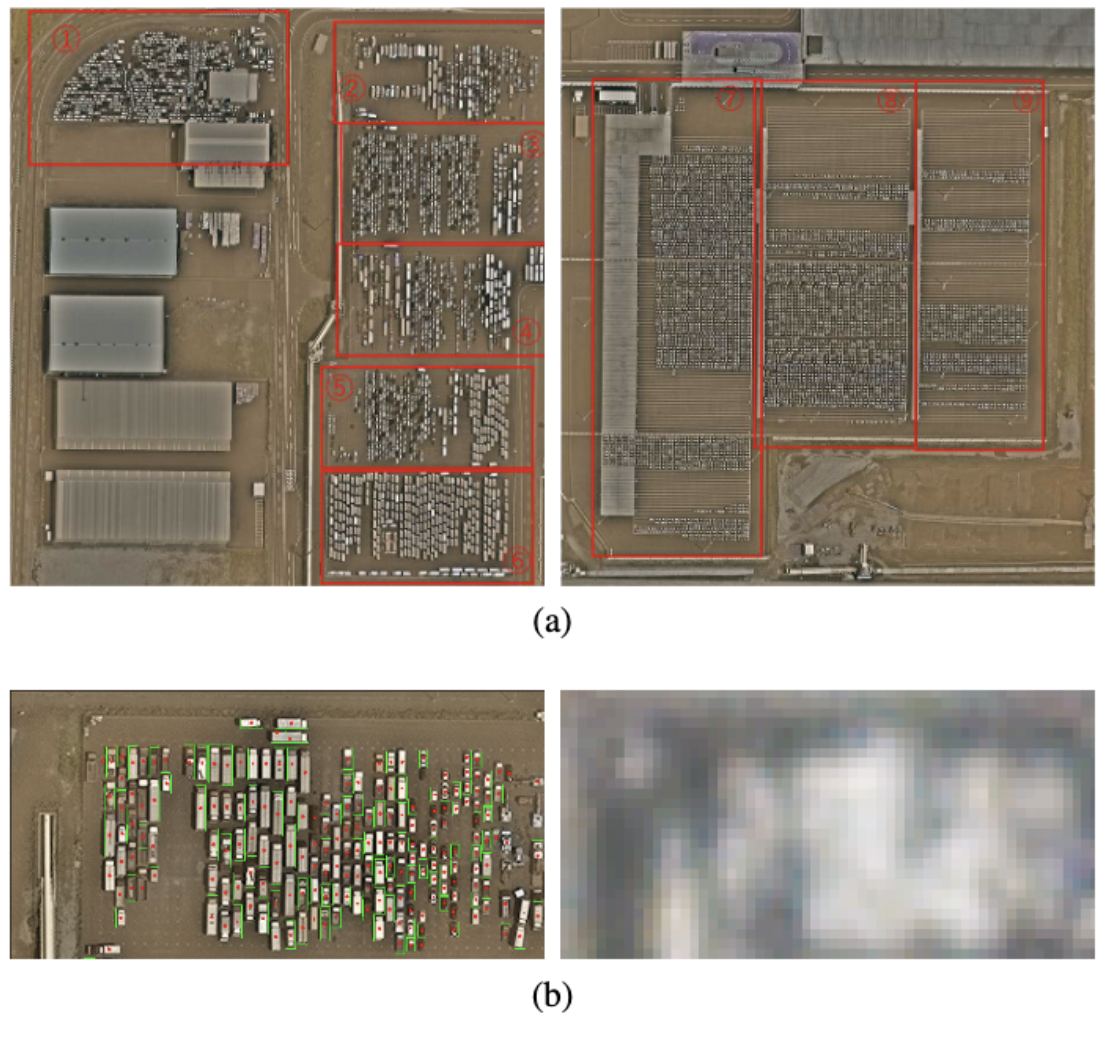
\includegraphics[width=\textwidth]{9park.png}
    \caption{计数区域划分和HR、LR实例图像}
    \label{fig:park}
\end{figure}

低分辨率图像可以分为两类,有对应高分辨率图像的和没有对应高分辨率图像的。对于前者而言,直接从对应高分辨率标注结果中计算覆盖率即可。那些没有HR图像对应的LR图像则由多名专家进行视觉标注并取平均值。
\subsection{空间一致性}  
通过上述对数据集的分析,我们可以看到高分辨率图像和与其对应的低分辨率图像之间间隔时间不大,同时对应的是同一位置。因此我们可以认为在它们上进行的目标计数结果应当也相同。两者所映射的空间信息应该具有一致性,这也给后续处理方法提供了思路。如何应用高分辨率图像信息指导改进低分辨率图像上估计的结果成为提高估计精度的关键节点之一。
\subsection{时间连续性}
单一的低分辨率图像很难得出合理的目标计数估计,然而由于低分辨率遥感图像的短重访周期,我们能得到一段连续的低分辨率图像。比较相邻图像间的变化或者从多个图像间进行学习,可以补充那些单张图像因低分辨率造成的信息缺失。图像间的时间连续性也是指导改进图像计数估计结果的关键因素。
\section{CRVC网络}
CRVC网络是针对CRVC数据集设计的深度学习模型。它以U-Net模型为骨架,设计了跨分辨率空间CRVC数据集中的跨分辨率空间信息和时序信息。通过上述网络估计出密度分布后,使用线性回归模型得出最终目标计数结果。
\subsection{网络设计}
\begin{figure}[h]
    \centering
    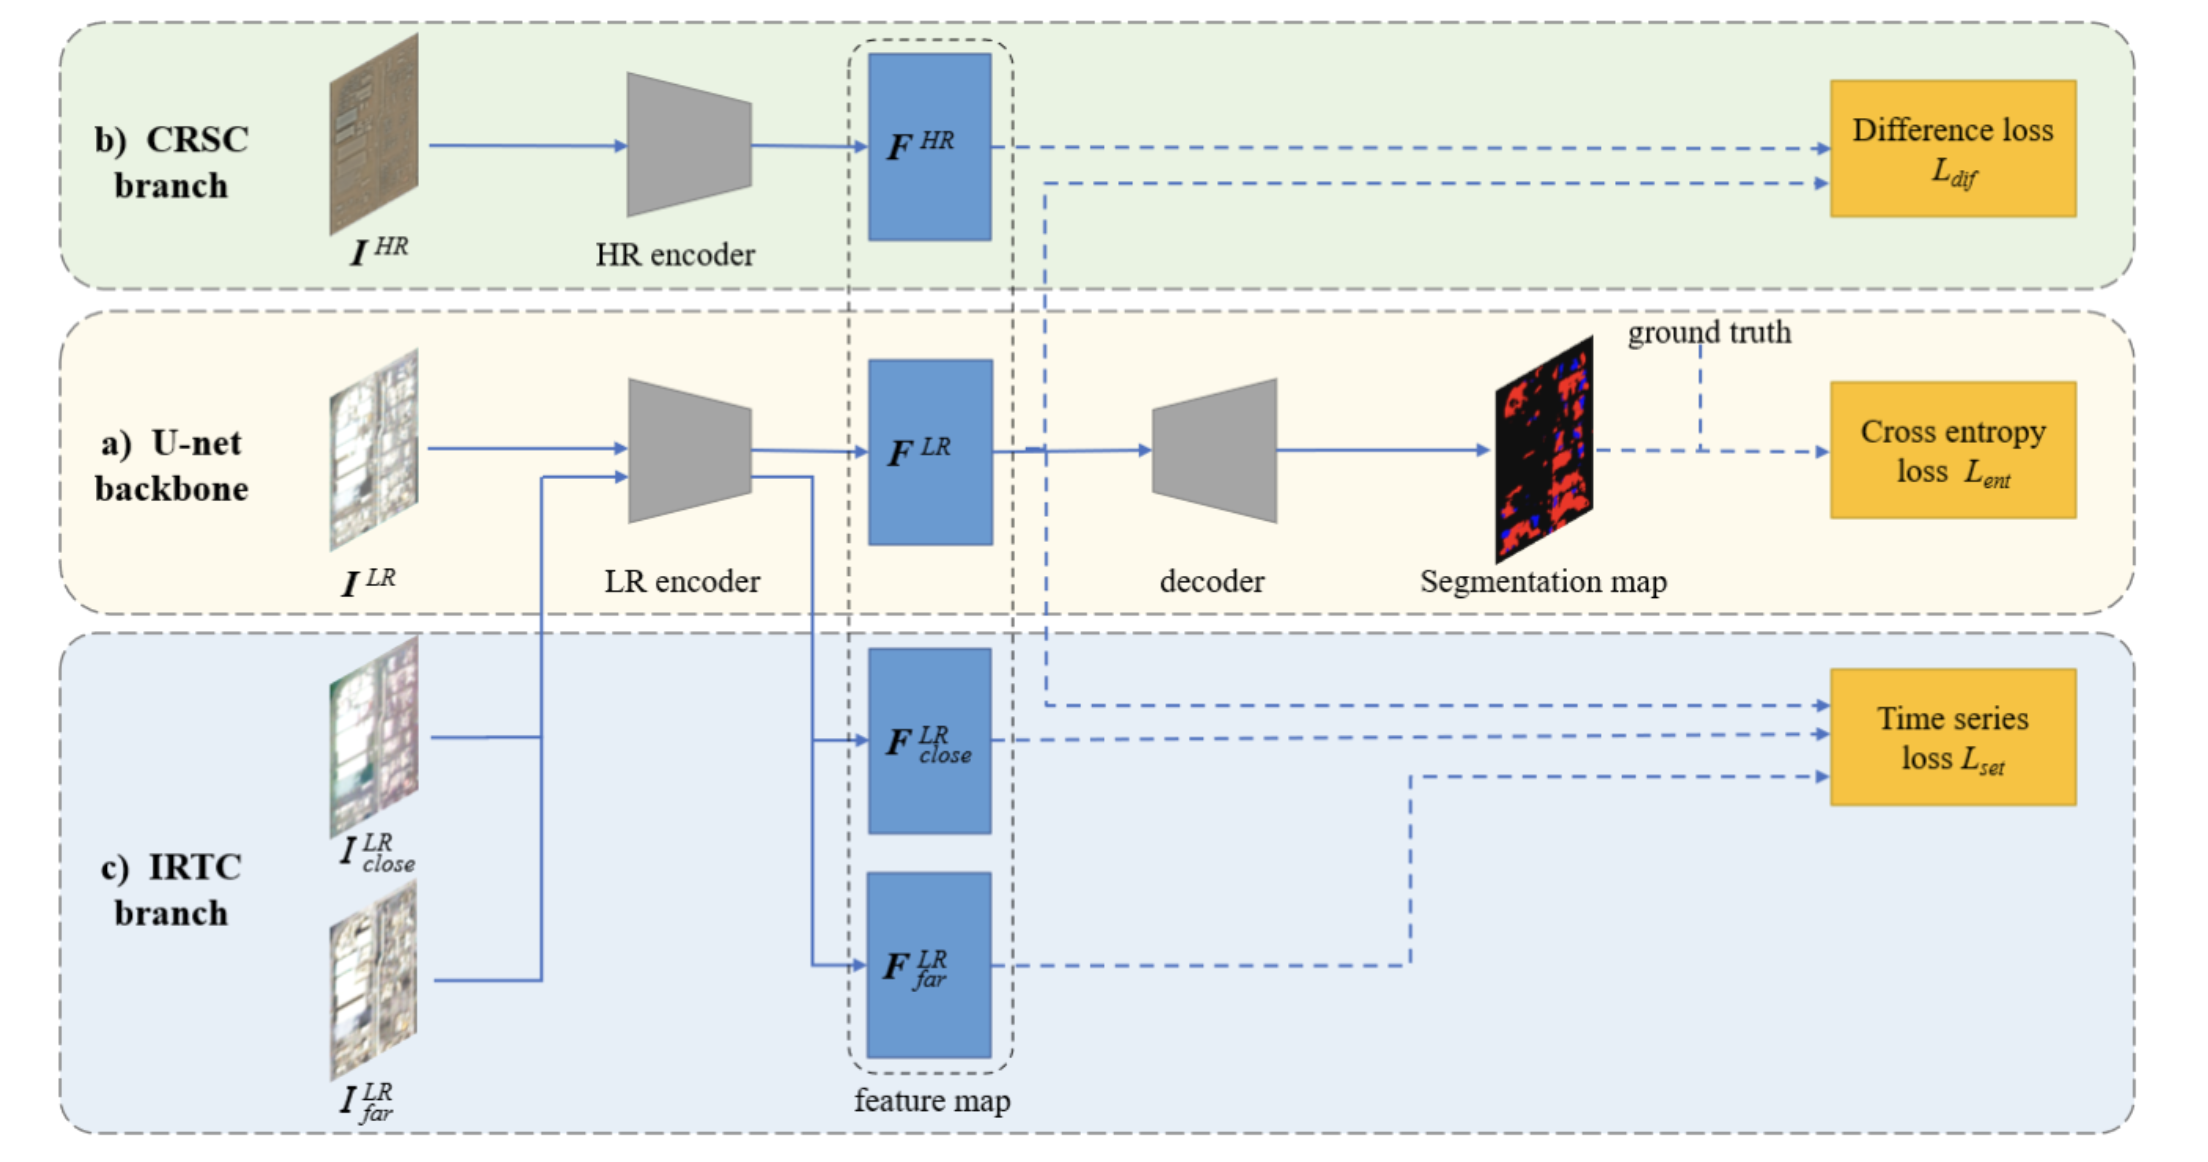
\includegraphics[width=\textwidth]{CRVCnet.png}
    \caption{CRVC网络架构}
    \label{fig:CRVCnet}
\end{figure}

上图~\ref{fig:CRVCnet}展示了模型的基本框架。模型接受4个输入,分别是高分辨率图像输入$I^{HR}$,对应低分辨率图像输入$I^{LR}$,与LR图像时间间隔较近的$I^{LR}_{near}$和与LR图像时间间隔较远的$I^{LR}_{far}$。模型包含两个独立学习的编码器HR encoder和LR encoder,前者用来提取高分辨率图像的特征,后者用来提取3个低分辨率图像的特征。提取出的低分辨率特征和高分辨率特征作差来综合更高精度的信息。之后通过带有跳跃连接的decoder完成分割图的生成。
\subsection{损失函数}
CRVCnet设计了三个损失函数,综合三个损失函数的结果来训练模型。
第一个损失函数为交叉熵损失函数,这个函数常用来衡量概率之间的距离。网络经sigmod输出的分割图也是一种概率分布。用交叉熵衡量其偏差程度有着不错的效果。
\begin{equation}
    \mathcal{L}_{\text {ent }}=-\frac{1}{n} \sum_{i} y_{i} \ln a_{i}
\end{equation}
对于高分辨率和低分辨率图像间的空间一致性,它们之间的差异越小,模型对于真实情况的把握就越好。文章提出了下面的损失函数进行约束。
\begin{equation}
    \mathcal{L}_{\text {dif }}=\sum_{i}\left|F_l^{L R}-F^{HR}_{l}\right|^2
\end{equation}

网络接受3个低分辨图像,分别是有高分辨率对应的低分辨率图像,距离这个低分辨率图像时间较近的图像和距离这个低分辨率图像时间较远的图像。由于时间连续性的约束,日期接近的图像间的差异应该小于日期相隔较远的差异。因此这部分损失函数的设计要求相邻日期图像间的差异更小,日期间隔较远的差异较大。下面的公式同时满足上述条件,且符合最小化损失的要求
\begin{equation}
    \mathcal{L}_{\text {ser }}=\sum_{l=1}^{m} \frac{\left|F_{\text {closel }}^{L R}-F^{L R}{ }_{l}\right|}{\left|F_{\text {far } l}^{L R}-F^{L R}_ l\right|}
\end{equation}
最终的损失函数由各个损失函数加权得到,即
\begin{equation}
    \mathcal{L}=\omega_1\mathcal{L}_{\text {ent }}+\omega_2\mathcal{L}_{\text {dir }}+\omega_3\mathcal{L}_{\text {ser }}
\end{equation}

其中$\omega_1,\omega_2,\omega_3$为各个损失函数的权重,是设定好的超参数。m是特征图的通道数.

\subsection{回归模型}

在CRVC数据集中,车辆在目标区域是密集停放的,而且不存在重叠。因此从分割图上估计出的覆盖率和最终的车辆数目具有线性关系。通过CRVC网络得到的覆盖率分割图,根据低分辨率图像的缩放比例,可以估计出实际面积。通过线性回归,找出参数k来拟合
\begin{equation}
    Number_i=k_i\dots Area_i+b_i
\end{equation}
其中i表示第i类车辆。这些参数通过高分辨率图像的真值计算得到。

% Chapter 4

\chapter{基于注意力机制的跨分辨率遥感影像计数}
在本节中,将详细介绍一种全新的基于注意力机制的跨分辨率遥感影像计数方法。通过分析CRVC数据集中数据的时间连续性和空间一致性特性,在现有网络基础上,设计了跨分辨率空间注意力和低分辨率下的时空注意力模块,充分结合了图像中的不同尺度,位置信息。
\section{问题分析}
由于直接从极低分辨率的图像中识别出车辆目标具有相当大的难度,本文通过将车辆计数问题转化为图像分割和回归问题来解决这一挑战。这种转换使得处理变得更为可行,是因为不论图像分辨率如何变化,同一类别的车辆数量与车辆实际占用面积之间的线性关系是恒定的。通过数据集中高分辨率图像的计数结果作为同一天同一地点的低分辨率图像的真值是有效的,同时解决了无法直接在低分辨率图像上人工计数得到真值的问题。车辆面积的计算需要基于车辆覆盖率(在图像中的车辆区域百分比)。为了计算车辆覆盖率,我们首先需要通过图像分割技术准确地从低分辨率图像中提取出车辆区域。因此,本文提出的车辆计数大致流程如下:
\begin{enumerate}    
\item 跨分辨率图像处理:我们将选择性地输入高分辨率图像以及与该高分辨率图像同一天的低分辨率图像,同时还包括距离该日期较近和较远的两张低分辨率图像。这些图像被输入到我们精心设计的分割网络中,该网络专门针对从极低分辨率图像中有效分割车辆区域进行了优化。
\item 车辆覆盖率的计算:通过应用先进的图像处理算法,网络将输出车辆的分割图。这些分割图将用于计算每个车辆的覆盖率,即每辆车在图像中所占的面积与整个图像面积的比例。
\item 车辆面积的转换与回归分析:将得到的车辆覆盖率转换为实际车辆面积,这一步是通过与车辆实际占用面积和数量之间的已知线性关系相结合完成的。我们将使用从高分辨率图像中得到的数据来计算回归模型的系数,这些系数反映了车辆面积与车辆数量之间的关系。然后,这些回归模型系数被应用到低分辨率图像上,以估计出车辆的数量。
\end{enumerate}
通过上述流程处理,即使这些低分辨率图像在视觉上难以分辨车辆细节,我们也能够参照高分辨率图像在极低分辨率图像中有效地进行车辆计数。此方法不仅提高了车辆计数的准确性,还为处理其他低分辨率图像分析任务提供了可能的方法论指导。
\section{网络设计}
网络设计如图8所示,网络基于CRVC-Net骨干网络搭建,采用U-Net编码器解码器结构。对于目标低分辨率图像,通过多层卷积网络组成的编码器提取出特征,用作后续解码器输入的一部分。在该编码器结构中,同时保留各层的中间结果,以便后续解码器中对应层使用。

为了利用来自高分辨率图像的先验空间信息和来自其他低分辨率图像的时间连续性约束,引入了两个监督分支跨分辨率空间一致性分支CRSC(crossresolution spatial consistency) 和同分辨率下时间一致性分支IRTC(intraresolution time continuity)。CRSC分支采用和主干编码器相同的架构,提取来自相应高分辨率图像的特征,以使同一天高分辨率图像和低分辨率图像的提取特征尽可能相似。IRTC分支共享主分支的模型及参数,提取来自距离该日期较近和较远的两张低分辨率图像的特征,后续将比较他们和主分支输出的差异。这是因为编码器应具有提取同一分辨率下所有图像的能力,而对于不同分辨率图像来说,像素密度不同导致图像细节不同,采取独立训练的编码器能更好表征不同细节特征,避免造成高分辨率图像细节的丢失,从而影响其指导能力。解码器接受主分支特征作为输入,同时在每一层解码器处,使用对应层的主分支及近处和远处低分辨率图像和高分辨率图像的中间结果作为key,设计了专门的注意力门,综合多渠道输入,进行解码。逐层操作直至生成分割图像。
\section{编码器}

\section{多来源注意力机制}
注意力机制有助于掌握时序信息,同时对于综合不同特征间相关关系有着很强的综合能力。本文中就针对CRVC数据集的特点,设计了自注意力门 SAG(Self Attention Gate)、跨分辨率注意力门 CAG(Crossresolution Attention Gate)和时间序列注意力门 TAG(Timeseires Attention Gate)三种注意力门模块,来充分利用数据集中的时间一致性和空间连续性特征。

如第二章所述,注意力机制主要需要三个输出,分别为key,query和value,通过下述公式可计算得出:
\begin{equation}
\text{Attention}(Q, K, V) = \text{Softmax}\left(\frac{QK^T}{\sqrt{d_k}}\right)V 
\end{equation}

首先是自注意力门,用主分支编码器对应中间层的结果作为key,解码器上一层上采样结果作为query和value进行计算。
跨分辨率注意力门,用CRSC分支编码器对应中间层的结果作为key,解码器上一层上采样结果作为query和value进行计算。
时间序列注意力门,用两个IRTC编码器对应中间层的结果分别作为key,解码器上一层上采样结果作为query和value进行计算。
\begin{figure}[h]
    \centering
    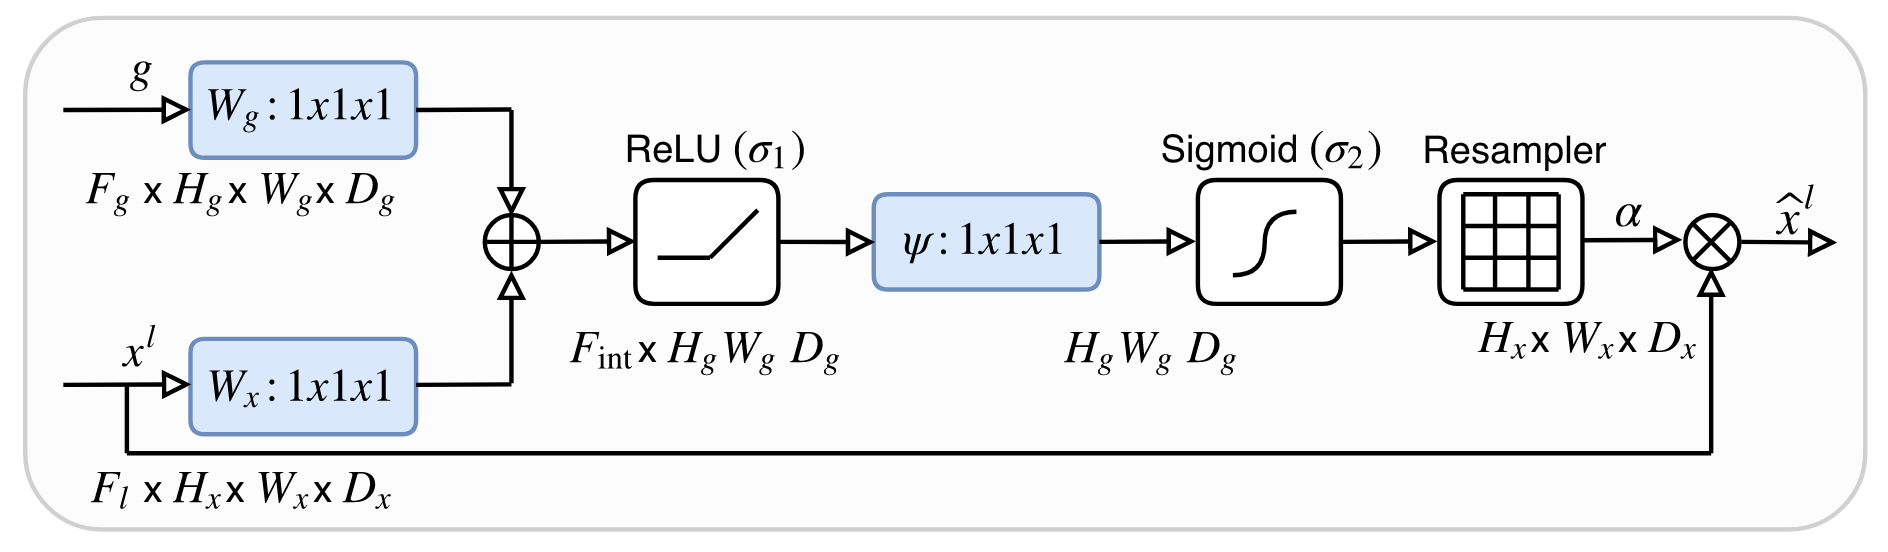
\includegraphics[width=\textwidth]{attentionG.png}
    \caption{U-Net网络结构}
    \label{fig:UNet}
  \end{figure}
本设计使用主分支、CRSC分支和IRTC分支分别作为key对解码器上一层上采样后的输出进行注意力操作。这种设计可以更精细地控制不同分支对最终输出的贡献,从而提升模型的性能和泛化性。

具体步骤如下
\begin{enumerate}    
    \item 获取Key和Query:Key来自于主分支、CRSC分支和IRTC分支的特征图。 Query则来自于解码器上一层的输出。
    \item 计算注意力权重: 使用query与每个key进行点积(或其他相似度计算方法),然后应用softmax函数来获取注意力权重。
    \item 应用注意力权重:使用得到的注意力权重对各分支的特征图进行加权求和,生成加权的特征图。
    \item 融合和上采样:将加权的特征图输入到解码器的当前层,进行上采样和进一步的处理。
\end{enumerate}

本文设计的网络将主分支、CRSC分支和IRTC分支编码器的对应层的中间结果分别用作注意力机制中的key,而对应的query和value则均来自上一层解码器的输出。这种设计允许模型在每一步解码过程中都重新评估各个编码器分支的重要性,更加动态地融合信息。此方法允许模型根据解码器的当前状态动态调整各个分支的权重,在反向传播中加以修改优化。同时通过考虑来自不同时间和空间信息的多个分支,模型能够更全面的利用数据集中的全部信息。

\section{解码器}

\section{损失函数}
与CRVC-Net类似,本设计中也包含其中的三个损失函数,不同的是本设计中额外使用焦点损失(Focal Loss)作为交叉熵函数的补充。

对于高分辨率和低分辨率图像间的空间一致性,使用下面的损失函数进行约束。
\begin{equation}
    \mathcal{L}_{\text {dif }}=\sum_{i}\left|F_l^{L R}-F^{HR}_{l}\right|^2
\end{equation}

对于时间连续性的约束,日期接近的图像间的差异应该小于日期相隔较远的差异。使用下面的损失函数进行约束。
\begin{equation}
    \mathcal{L}_{\text {ser }}=\sum_{l=1}^{m} \frac{\left|F_{\text {closel }}^{L R}-F^{L R}{ }_{l}\right|}{\left|F_{\text {far } l}^{L R}-F^{L R}_ l\right|}
\end{equation}

\subsection{焦点损失函数}
焦点损失函数(Focal Loss)最初是为解决目标检测中的类别不平衡问题设计的,尤其是在目标识别中背景与前景类别之间的不平衡问题。然而,这种损失函数的设计原理使其同样适用于广泛的多分类问题,特别是在存在明显类别不平衡的情况下。对于包含多种车辆类型的CRVC数据集,各类车辆数量极不平衡,其中包括轿车35844辆、小型货车737辆、大型货车1211辆、起重机60辆。 如果数据集中某些类型的车辆比其他类型少得多,使用焦点损失函数可以带来明显的优势。由于轿车数量显著多于其他几类车辆,采用交叉熵函数时
\begin{equation}
    \mathcal{L}_{\text {ent }}=-\frac{1}{n} \sum_{i} y_{i} \ln a_{i}
\end{equation}
其中的轿车样本占大多数,将显著影响损失函数整体的值,而缩小其他类别对于损失函数的贡献。因此在最终得到的网络中,对于其他几类的分类效果也因此受到影响。


焦点损失函数是交叉熵损失函数的一种改进。焦点损失函数通过重新设计交叉熵损失,可以调节不同数量样本之间的权重,从而使模型对于少量样本的表示能力更强,从而提高模型整体性能。


焦点损失函数的定义如下:
\begin{equation}
    FL(p_t) = -\alpha_t (1 - p_t)^\gamma \log(p_t)
\end{equation}

其中:\( p_t \) 是模型对当前样本的预测概率,对于正样本 \( p_t = p \),对于负样本 \( p_t = 1 - p \)。 \( \alpha_t \) 是平衡正负样本权重的系数,通常设置为一个小于 1 的值,用来增加少数类的重要性。\( \gamma \) 是调整易分类样本对损失的影响的聚焦参数,\( \gamma \geq 0 \)。当 \( \gamma = 0 \) 时,Focal Loss 退化为标准的交叉熵损失。\( \gamma \) 的值越大,对易分类样本的惩罚就越大。


通过引入调制因子 \( (1 - p_t)^\gamma \):当一个样本被错误分类,并且错误程度很大(即 \( p_t \) 很小)时,\( (1 - p_t)^\gamma \) 接近 1,损失不受影响。当一个样本被正确分类,且分类器置信度很大时(即 \( p_t \) 很大)时,\( (1 - p_t)^\gamma \) 接近 0,这使得这类样本对总损失的贡献大大降低,这样可以让模型集中精力学习那些难以分类的样本。


在多分类问题中,焦点损失函数的应用类似于其在二分类中的用法,但需要一些调整来处理多个类别。多分类版本的焦点损失函数通常表示为:

\begin{equation}
    FL(p_t) = - \sum_{c=1}^C \alpha_c (1 - p_{t,c})^\gamma \log(p_{t,c})
\end{equation}


其中:
\( C \) 是类别的总数。\( p_{t,c} \) 是模型对于每个类别 \( c \) 的预测概率。如果样本属于类别 \( c \),则 \( p_{t,c} \) 是该类别的预测概率;否则为 \( 1 - p_{t,c} \)。\( \alpha_c \) 是针对类别 \( c \) 的平衡系数,用于调节不同类别间的不平衡。\( \gamma \) 是聚焦参数,用来减小易分类样本的损失贡献,增加难分类样本的影响。


通过调节 \( \alpha_c \) 和 \( \gamma \) 参数,焦点损失函数可以帮助模型更好地学习那些样本数量较少的类别。这是通过增加这些类别样本的损失贡献来实现的,从而使模型在训练过程中更加关注它们。通过 \( (1 - p_{t,c})^\gamma \) 这一调节项,焦点损失函数提高了那些模型难以正确分类的样本的损失权重,从而激励模型改进这些区域的预测性能。


对于一个批次中的所有样本,焦点损失函数完整的表达式通常写作:

\begin{equation}
    \mathcal{L}_{\text {FL}} = -\frac{1}{N} \sum_{i=1}^{N}\sum_{c=1}^C \alpha_c (1 - y_{i,c})^\gamma \log(y_{i,c})
\end{equation}


其中:\(N\) 是批次中样本的总数。\( C \) 是类别的总数。\(i\) 是批次中的样本索引。\(y_{i,c}\) 是第 \(i\) 个样本的为类别\( c \)的预测概率,\(\alpha_t\) 是一个调制因子,用于平衡正负样本之间的影响。\(\gamma\) 是一个调整参数,用于减少易分类样本的权重。



最终的损失函数由各个损失函数加权得到,即
\begin{equation}
    \mathcal{L}=\omega_1\mathcal{L}_{\text {ent }}+\omega_2\mathcal{L}_{\text {dir }}+\omega_3\mathcal{L}_{\text {ser }}
    +\omega_4\mathcal{L}_{\text {FL }}
\end{equation}

其中$\omega_1,\omega_2,\omega_3,\omega_4$为各个损失函数的权重,是设定好的超参数。

% Chapter 5
\chapter{跨分辨率遥感影像计数实验及分析}
\section{实验设计}
本设计探究的是跨分辨率遥感影像的计数问题,在跨分辨率车辆计数数据集上,训练本文设计的网络,测试其性能。数据集中共包含了拍摄于同一位置不同时间的192 张极低分辨率图像和 8 张高分辨率图像,低分辨率图像中包含8张和高分辨率图像再同一天拍摄的图像。如何通过少量的高分辨率图像的计数结果,得到可以在低分辨率图像上做出准确计数估计的模型就是本设计的目标。本设计基于CRVC-Net骨架网络,通过独特设计的3个注意力门,更好的综合了从高分辨率及其余两个时间的低分辨率图像的特征信息,逐层与解码器输出进行计算,改进输出效果。

\section{模型训练}
在训练阶段,四张图像输入到网络中。第一输入是\( I^{LR}\),低分辨率图像用于在骨架中生成车辆分割。第二输入是相应的高分辨率图像\( I^{HR}\),起到空间引导的作用。\( I^{LR}\)和\( I^{HR}\)应该在8对相应的低分辨率和高分辨率图像中选取。我们使用其中的7对进行训练,1对进行测试。第三和第四输入是一对低分辨率图像,即\( I^{LR}_{close}\)和\( I^{LR}_{far}\),以强调时间连续性。\( I^{LR}_{close}\)选为与\( I^{LR}\)日期最接近的图像,而\( I^{LR}_{far}\)在图像集中随机选取,与\( I^{LR}\)的时间差超过50天。由于低分辨率和高分辨率图像对数量较少,为了增强鲁棒性,将训练图像裁剪为32×32的补丁后,通过旋转90度、180度和270度,上下左右翻转,将训练集扩大至4000个图像补丁。测试集扩增到1000个图像补丁。在解码器的上采样过程中,使用U-Net结构将上采样的图像与相应比例的特征图跳跃连接。网络输出与原始图像补丁大小相同的32×32的最终分割图。由于训练集是通过旋转和翻转方法生成的,最终的分割结果应该是来自同一图像的各种增强图像的平均值。然后将32×32的补丁拼接成所需的图像大小,以获取整个停车场区域的图像。在测试阶段,只需将\( I^{LR}\)输入到分割骨架中,输出即为车辆分割图。考虑到起重机的数量太少,对分割结果影响不大,我们排除了这一类别,训练和测试阶段只涵盖轿车、小型货车、大型货车和背景四类。

本方法先得到从低分辨率图像得到的分割图,然后据此估计出覆盖率,再由覆盖率通过回归模型估计出最总计数结果,因此主要从以下三个维度度量模型性能:
\begin{enumerate}    
    \item 测试模型在低分辨率(LR)图像上的分割结果,与相应的高分辨率(HR)图像的真实标注进行比较。
    \item 在所有低分辨率图像上测试的车辆覆盖率结果,与人工标注进行比较。
    \item 测试模型在低分辨率图像上的计数结果,与相应高分辨率图像的真实标注进行比较。
\end{enumerate}

\section{分割精度测试}
以同一日期的高分辨率图像的分割图作为标注,本设计在各种网络模块的组合上测试了分割精度。采用像素精度(Pixel Accuracy,PA)来定量评估分割精度。它表示所有像素中正确分类的比例。
\begin{equation}
    P A=\frac{\sum_{i}^{k} p_{i i}}{\sum_{i}^{k} \sum_{j}^{k} p_{i j}}
\end{equation}

假设有\(k+1\)个类别(包括\(k\)个目标类别和1个背景类别),\(p_{ij}\)表示属于类别i但被预测为类别j的像素数量。因此\(p_{ii}\)代表类别为i预测结果也为i的真阳性(TP),\(p_{ij}\)代表类别为i预测结果也为i的假阳性(FP),\(p_{ji}\)代表类别为i预测结果也为i的假阴性(FN)。
基于真阳性(TP)、假阳性(FP)和假阴性(FN),为了更全面的度量该方法在分割方面的性能,通过使用了如召回率(Recall)、精确度(Precision)和F1分数等指标来进一步指示估计精度。\begin{equation}
    \text { Recall }=T P /(T P+F N)
\end{equation}
\begin{equation}
    \text { Precision }=T P /(T P+F P) 
\end{equation}
\begin{equation}
    F 1=2 T P /(2 T P+F P+F N)
\end{equation}结果列在表~\ref{tab:evaluation}中。本文的方法在召回率、精确度和F1分数上均有一定提高。
\begin{table}[h]
    \centering
    \caption{召回率、精确度和F1分数}
    \label{tab:evaluation}
    \begin{tabularx}{\textwidth}{CCCCCCC}
      \toprule
      模型 & 真阳性 & 假阴性 & 假阳性  & 召回率 & 精确度 & F1分数   \\
      \midrule
      CRVC-Net   & 2027  & 2194 & 1037 & 48.0\% & 66.2\% & 0.556 \\   
      本文模型   & 2134  & 2149 & 975 & 49.8\% & 68.6\% & 0.577 \\   
      \bottomrule
    \end{tabularx}
\end{table}


\subsection{消融实验}
为了验证并解释模块设计的合理性和因果性,针对3种注意力门设计了消融实验。
\begin{enumerate}    
    \item 仅使用CRVC-Net骨架进行训练。
    \item 仅使用自注意力门的CRVC-Net进行训练。
    \item 仅使用跨分辨率注意力门的CRVC-Net进行训练。
    \item 仅使用时间序列注意力门的CRVC-Net进行训练。
    \item 使用自注意力门和跨分辨率注意力门的CRVC-Net进行训练。
    \item 使用自注意力门和时间序列注意力门的CRVC-Net进行训练。
    \item 使用自注意力门、时间序列注意力门和跨分辨率注意力门的CRVC-Net进行训练。
\end{enumerate}
实验的结果如下表所示:
\begin{table}[h]
    \centering
    \caption{注意力门消融实验}
    \label{tab:attentiongate}
    \begin{tabularx}{\textwidth}{CCCCC}
      \toprule
      模型 & 自注意力门SAG & 跨分辨率注意力门CAG & 时间序列注意力门TAG & 像素精度  \\
      \midrule
      CRVC-Net   & \times  & \times & \times & 87.5\% \\
      base+SAG   &\surd   & \times & \times & 87.7\% \\     
      base+CAG   & \times  & \surd & \times & 86.3\% \\     
      base+TAG   & \times  & \times & \surd & 84.8\% \\     
      base+SAG+CAG   & \surd  & \surd & \times & 88.2\% \\     
      base+SAG+TAG   & \surd  & \times & \surd & 87.4\% \\     
      base+SAG+CAG+TAG   & \surd & \surd & \surd & \textbf{88.4\%}  \\     
      \bottomrule
    \end{tabularx}
\end{table}

\subsection{实验结果分析}
从上表~\ref{tab:attentiongate}我们可以发现,单独增加自注意力门可以提升像素估计精度,但单独增加跨分辨率注意力门和时间序列注意力门却对估计精度有负面影响。这可能是因为单独引入高分辨率分支特征虽然在训练集上有助于提升最终估计效果,但对于低分辨率的图像的泛化性能却有所下降。单独引入时间序列注意力门虽然丰富了解码器的输入,但没有高分辨率参照下的其余低分辨率特征,并不能很好的指导模型做出正确的估计,反而影响了模型的性能。同时引入自注意力门和跨分辨率注意力门比较明显的提升了模型的性能,同时引入自注意力门和时间序列注意力门也较先前模型有了明显的提升。同时使用三种注意力门单元的模型取得了最好的像素精度估计,也证明了时间序列注意力门单元设计的有效性。虽然单独添加TAG门的效果不佳,但其作为完整模型的一部分有效的弥补了对于不同时间的低分辨率图像的识别能力的不足。
\section{覆盖率估计测试}
在上一步骤中,通过网络模型可以得到低分辨率图像的分割图像估计,据此可以得出车辆的覆盖率。但是由于只有少量低分辨率图像有对应的高分辨率图像作为标注,大部分低分辨率图像采用人工专家标注的方法来判断模型估计的覆盖率结果。低分辨率图像的覆盖率以5\%的间隔手工标注。考虑到人工标注可能存在一些错误,我们根据两个标注者的标注结果的差对标注进行了一些预处理:差值不超过5\%的标注被认为是准确的,而差值位于10\%左右被认为是可接受的。如果差值大于15\%,则认为发生了来两者标注中可能存在错误,将该值排除并由其他专家进行重新标注。上述规则确保了标签的可信度。然后,使用所有人的平均标签值来评估车辆覆盖估计的准确性。下图~\ref{fig:seg}展示了模型估计覆盖率和人工标注覆盖率。
\begin{figure}[h]
    \centering
    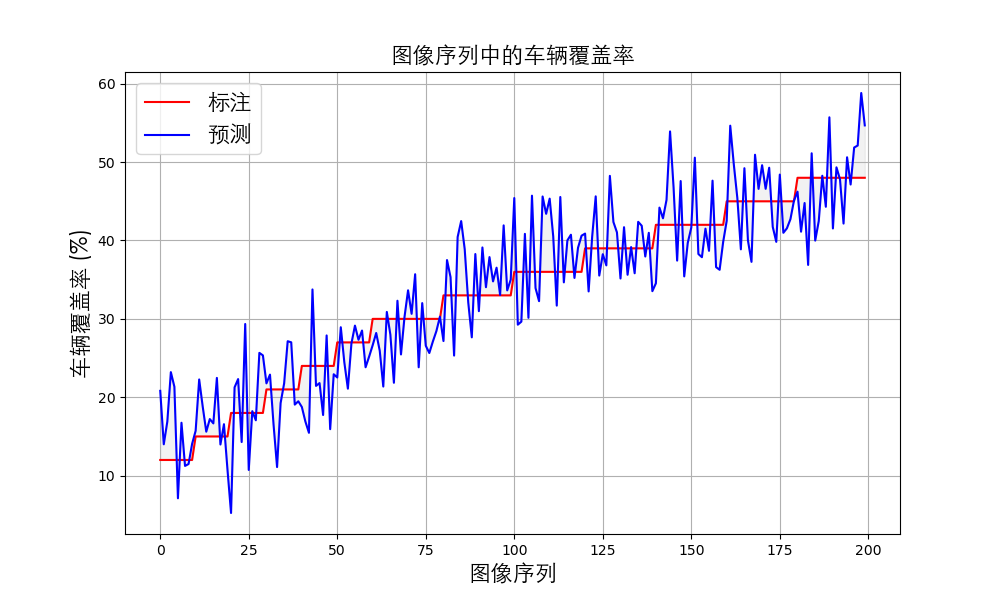
\includegraphics[width=\textwidth]{segmentation.png}
    \caption{覆盖率估计}
    \label{fig:seg}
\end{figure}

\section{车辆计数回归结果测试}
通过车辆覆盖率,可以通过低分辨率图像的大小来计算出车辆区域面积。通过高分辨率图像提供的真值计数信息,可以进行回归分析。本文中对四个车辆类别分别进行了车辆区域面积和车辆数目的回归分析,得到的结果如下图所示。
\begin{figure}[h]
    \centering
    % 第一行两张图
    \begin{subfigure}{0.45\textwidth}
      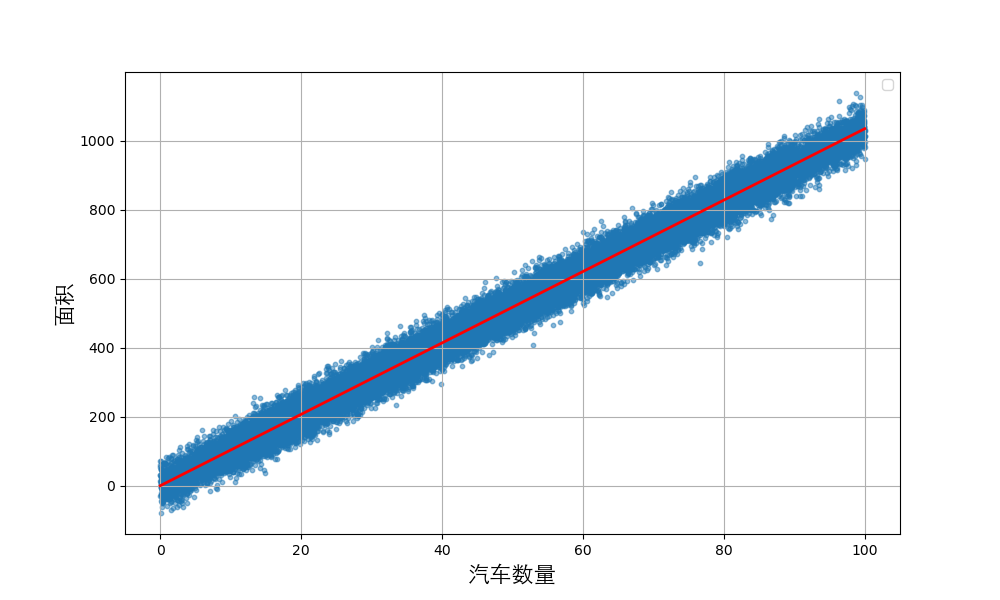
\includegraphics[width=\linewidth]{cars.png}
      \caption{小汽车}
      \label{fig:subfig-a}
    \end{subfigure}\quad % 添加一些间隔
    \begin{subfigure}{0.45\textwidth}
      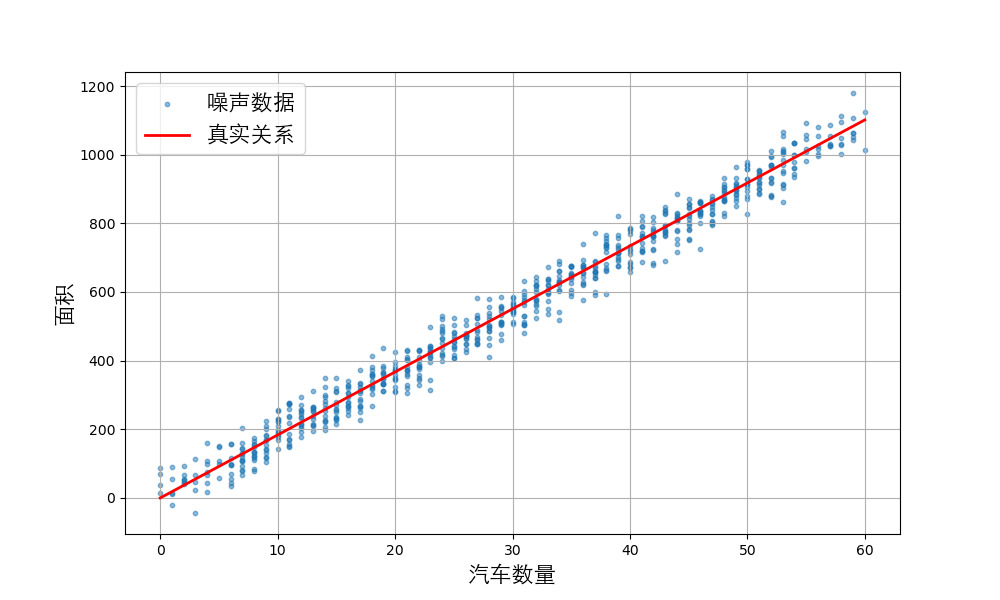
\includegraphics[width=\linewidth]{smalltrucks.png}
      \caption{小型货车}
      \label{fig:subfig-b}
    \end{subfigure}
  
    % 第二行两张图
    \begin{subfigure}{0.45\textwidth}
      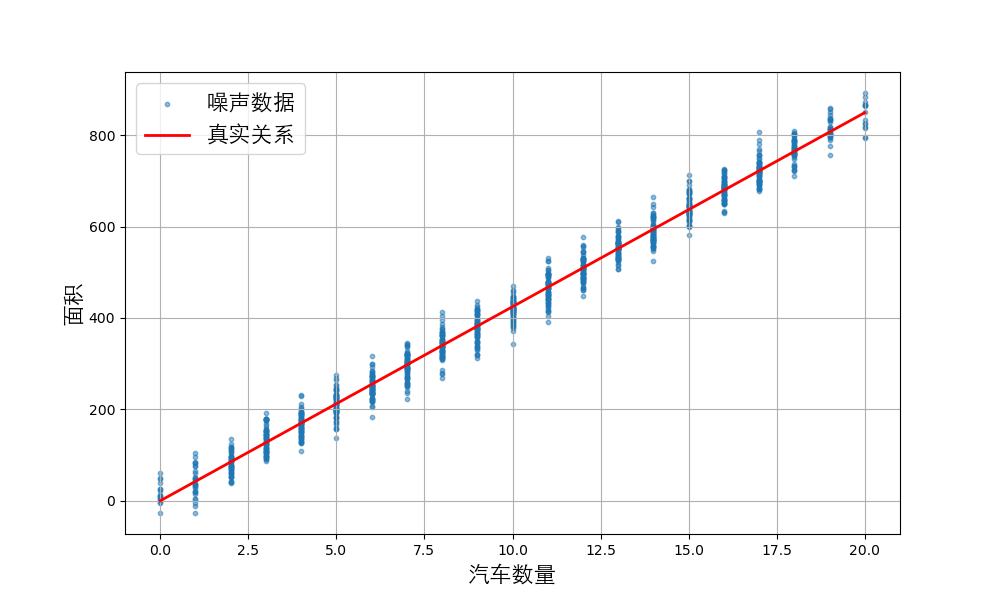
\includegraphics[width=\linewidth]{largetruck.png}
      \caption{大型货车}
      \label{fig:subfig-c}
    \end{subfigure}\quad % 添加一些间隔
    \begin{subfigure}{0.45\textwidth}
      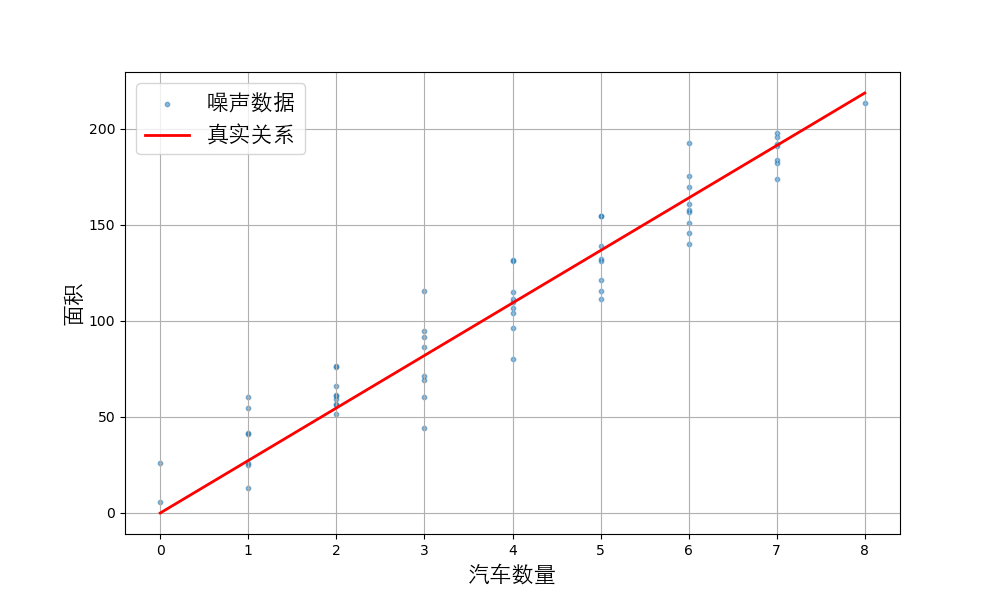
\includegraphics[width=\linewidth]{cranes.png}
      \caption{起重机}
      \label{fig:subfig-d}
    \end{subfigure}
  
    \caption{四种汽车回归计数的结果}
    \label{fig:multi-image}
\end{figure}

  对于小汽车、小型货车、大型货车和起重机四个类别,回归模型预测的斜率分别为10.353、18.354、42.468和27.323,\(R^2\)分别为0.9867、0.9821、0.9854和0.9376。\(R^2\)大于零且接近一,具有很强的正相关性。

\section{训练细节}
在训练过程中涉及到多个超参数的选择,其中比较重要的是损失函数的权重。模型使用的损失函数如下:
\begin{equation}
    \mathcal{L}=\omega_1\mathcal{L}_{\text {ent }}+\omega_2\mathcal{L}_{\text {dir }}+\omega_3\mathcal{L}_{\text {ser }}
    +\omega_4\mathcal{L}_{\text {FL }}
\end{equation}
为了能够让模型能够先掌握车辆的整体结构及更好的适应数量占据大多数的轿车类别,在前10000个轮次中,将\(\omega_4\)设置为0,将\(\omega_1\)设置为0.5,将\(\omega_2\)设置为0.4,将\(\omega_3\)设置为0.1,以避免对于轿车分类的惩罚。在后续的5000个轮次中,\(\omega_1\)设置为0,\(\omega_2\)和\(\omega_3\),\(\omega_4\)设置为0.5,这时使用焦点损失函数专注于学习大型货车和小型货车类别。这有助于更好的识别小样本类别,同时对于背景类别的也能有更好的区分


\section{局限}
本模型采用的多头注意力门结构确实可以增加模型对数据的理解深度,但同时也会带来一系列局限性和挑战。

首先多头注意力机制通常会导致显著的参数增加。这种参数增加意导致在训练和推理过程中需要更多的内存来存储额外的参数和中间计算结果。这种增加的内存需求可能会限制模型能够处理的最大批量大小。当该方法应用于其他更大规模的数据集上时,参数量及训练时间的影响将更为显著。下表展示了不同模型的参数数量对比,可以直观的观察出参数量的增长。
\begin{table}[h]
    \centering
    \caption{不同模型的参数量}
    \label{tab:parma}
    \begin{tabularx}{\textwidth}{CCCC}
      \toprule
      模型 & 总参数量 & 可训练参数量 & 内存占用  \\
      \midrule
    CRVC-Net& 37,922,787  & 37,916,773 & 144.66MB \\
    CRVC-Net+AG& 50,689,801  & 50,677,897 & 193.37MB \\
    本文模型  & 134,969,540    & 134,956,548 & 514.87MB \\   
      \bottomrule
    \end{tabularx}
\end{table}


参数数量的增加,尽管可以帮助模型学习更复杂的特征,但也可能使模型更容易过拟合,特别是在如CRVC这样的小型数据集上训练时。即使使用图像增广技术,如翻转、缩放和平移,这些操作可能不足以生成模型需要的多样化数据来充分学习并泛化到未见过的数据。
同时大量的参数和复杂的模型结构可能导致优化过程中出现问题,如梯度消失或梯度爆炸,对于参数的调整和优化算法的选择上有着更高的要求。






% Chapter 6

\chapter{总结与展望}
\section{结论}
本文设计了一种基于多头注意力机制的U-Net网络模型,同时使用焦点损失平衡类别数目不平衡的问题。本设计测试了该方法在跨分辨率遥感影像车辆计数问题上的准确性,尤其是对于稀少类别的估计准确率有不小的提升。模型通过实现不同的注意力门(自注意力门、跨分辨率注意力门、时间序列注意力门),展现了模型在处理复杂图像数据时的灵活性。通过设计消融实验,验证了各注意力门的重要性和影响,显示单独和组合使用各注意力门对模型性能的不同影响。最终实现的三种注意力门组合提供了最高的像素精度,说明了多头的注意力机制门的在综合时间连续性和空间一致性上的有效性。在训练过程中分阶段采用不同的损失函数,特别是引入了焦点损失,有效解决了类别分布不平衡的问题,在小型货车和大型货车的计数结果上取得了显著的提升。本文的研究成果不仅在车辆计数领域具有重要的应用价值,对于其他涉及到跨分辨率图像以及利用低分辨率图像的问题上,该模型也具有很强的迁移潜力。
\section{不足与展望}

本模型虽然在CRVC数据集上取得了不错的计数估计结果,但也仍存在一些不足之处。多头注意力机制虽然增强了模型的性能,但也大幅增加了参数数量,这导致更高的内存需求和可能的存在过拟合问题。高参数量和复杂的结构可能引起优化过程中的问题,如梯度消失或梯度爆炸,这要求更精细的参数调整和优化策略。同时CRVC数据集较小的数据量可能限制了模型的泛化能力,对于未见过的更大或更复杂的数据集,模型可能需要进一步的调整和优化。

本研究表明,虽然设计的模型在跨分辨率图像的车辆计数任务中表现出了良好的性能,但对于未来的工作,探索参数效率更高的模型架构、增强模型的泛化能力以及优化内存和计算资源的使用,将是进一步提升模型应用实用性的关键方向。进一步发掘高低分辨率图像间的隐含关系也将影响模型预测性能。


\end{document}